% Set document format
%%%%%%%%%%%%%%%%%%%%%%
\documentclass[a4paper]{article}
\usepackage[margin=2cm, left=2cm, right=3cm]{geometry}


% Set bibliography format
%%%%%%%%%%%%%%%%%%%%%%
% \usepackage[style=authoryear-comp, url=false, doi=true, isbn=false, maxcitenames=2, maxbibnames=30]{biblatex}
\usepackage[style=authoryear-comp]{biblatex}
% Remove "In" in the bibliography
\renewbibmacro{in:}{}
% Remove pp. in the bibliography
\DeclareFieldFormat{pages}{#1}
\addbibresource{references.bib}
\setcounter{biburlnumpenalty}{9000}
\setcounter{biburllcpenalty}{7000}
\setcounter{biburlucpenalty}{8000}

% Load relevant packages
%%%%%%%%%%%%%%%%%%%%%%
\usepackage{setspace} 
\usepackage{amsmath}
\usepackage[version=4]{mhchem}
\usepackage{siunitx}
\usepackage{authblk}
\usepackage{graphicx, wrapfig, rotating}
\usepackage[font=footnotesize]{caption}
\usepackage{float}
\usepackage{booktabs}
\usepackage[english]{babel}
\usepackage{enumitem}
\usepackage{abstract}
\usepackage[space]{grffile}
\usepackage[colorlinks=true, citecolor=green, linkcolor=black, urlcolor=blue]{hyperref}
\usepackage{acro}
\usepackage[T1]{fontenc}
\usepackage{lmodern}
\usepackage[normalem]{ulem}
\usepackage{makecell}
\usepackage{pdfpages}
\usepackage[section]{placeins}
\usepackage{tabularx}
    \newcolumntype{L}{>{\raggedright\arraybackslash}X}

\usepackage{todonotes}

\setlength{\parindent}{0em}
\setlength{\parskip}{1em}
\usepackage{xcolor}
\usepackage{caption}
\usepackage{subcaption}
\usepackage{tikz}
\usetikzlibrary{positioning,arrows.meta}

% Prime in author names of the reference library (Sobol')
\DeclareUnicodeCharacter{2032}{'}

% Table captions on top
\captionsetup[table]{position=top}

% The generated tables are copied into this file by src/make_results_figures.py, between the
% lines '% <<< generated: tab_name >>>' and '% <<< end of tab_name >>>': edit them through the script.


\def\UrlBreaks{\do\/\do-}

% Set Keyboards
%%%%%%%%%%%%%%%%%%%%%%
\providecommand{\keywords}[1]{\textbf{Keywords:} #1}

% Change name of Figures
%%%%%%%%%%%%%%%%%%%%%%%%
\addto\captionsenglish{\renewcommand{\figurename}{Fig.}}

% class `abbrev': abbreviations:
\DeclareAcronym{admlc}{
 short = ADMLC,
 long = After Diversity Mean Load Curve} 
\DeclareAcronym{dash}{
 short = DAVE,
 long = Dynamic anthropogenic activities and feedback to emissions} 
\DeclareAcronym{dave}{
 short = DAVE,
 long = Dynamic Anthropogenic actiVities and feedback to Emissions} 
\DeclareAcronym{dsm}{
 short = DSM,
 long = Demand Side Management} 
\DeclareAcronym{dsr}{
 short = DSR,
 long = Demand Side Response}
\DeclareAcronym{dvr}{
 short = DVR,
 long = Demand as Voltage control Reserve}
\DeclareAcronym{ev}{
 short = EV,
 long = Electric Vehicle}
\DeclareAcronym{hetus}{
 short = HETUS,
 long = harmonised time use surveys}
\DeclareAcronym{hvac}{
short = HVAC,
long = Heating Ventilation and Air Conditioning}
\DeclareAcronym{ict}{
 short = ICT,
 long = Information and Communication Technology}
\DeclareAcronym{pv}{
 short = PV,
 long = Photo-Voltaics}
\DeclareAcronym{tus}{
short = TUS,
long = time-use surveys}
\DeclareAcronym{v2g}{
short = V2G,
long = Vehicle-to-Grid}

% START DOCUMENT
%%%%%%%%%%%%%%%%%%%%%%%%%%%%%%%%%%%%%%%%%%%%%%%%%%%%%%%%%%%%%%%%%%%%%%%%%%%%%%%%%%%%%%%
%%%%%%%%%%%%%%%%%%%%%%%%%%%%%%%%%%%%%%%%%%%%%%%%%%%%%%%%%%%%%%%%%%%%%%%%%%%%%%%%%%%%%%%

\begin{document}

\pagenumbering{arabic}
\date{}
\author[1,2,*]{Samuele Lo Piano}

\affil[1]{\footnotesize{\textit{Faculty of Management and Economics, Gdansk University of Technology, Gdansk, Poland}}}
\affil[2]{\footnotesize{\textit{Barcelona School of Management, Universitat Pompeu Fabra, Barcelona, Spain}}}

\affil[*]{Corresponding author: Samuele Lo Piano, samuele.lo.piano@pg.edu.pl}


\title{Imputation of missing locations in time-use surveys}

\maketitle

\section*{Abstract}
Time-use diaries are a primary input to models of energy demand, which need to know not only people's activity but also their locations. The German contribution to the 2010 round of the Harmonised European Time Use Surveys (HETUS) records activities and trips but not the places where activities took place. We impute these places from the 13 HETUS countries that record all of them, assigning one location to each activity episode with a Markov chain that conditions on the activity, the time of day, the previous location, intervening trips and the respondent's age, with hierarchically smoothed probabilities. Imputing each of these countries from the other 12, the method recovers the recorded location in 87\% of ten-minute slots (Cohen's $\kappa$ 0.67), reproduces the share of people at home by time of day to within about 2.5 percentage points (pp) on average and keeps the number of location changes per diary close to the recorded one, which slot-by-slot imputation overstates sixfold. Assigning the most likely location raises accuracy to 91\% but overstates the time at home. When all modelling choices are varied together, two of them decide how good the imputed diaries are: whether a location is drawn at random or set to the most likely one, and whether locations are assigned to whole activity episodes in sequence or to each ten-minute slot. Adding the respondent's age or the day of the week, or changing the amount of smoothing, makes almost no difference. No combination of choices is best on every evaluation metric, and all Pareto-optimal ones use the Markov chain. The errors that remain are systematic: countries where people spend much time at second homes, such as Finland and Norway, are imputed with too much time at home. This error of transferring locations from one country to another accounts for most of the uncertainty of the German estimates of time spent at each place (92\% of the variance of the time at home), far more than the randomness of the draws or the modelling choices, and repeated imputations, as used in multiple imputation, do not reveal it. Only for the number of location changes do the modelling choices matter as much as the transfer error. For Germany, the method assigns 17.1 hours a day to the home, with 90\% of the combinations of choices, assumptions, random draws and transfer errors between 15.7 and 17.8 hours.

\section*{Highlights}
\begin{itemize}
    \item Activity locations missing from German HETUS diaries are imputed from 13 countries
    \item One location per activity episode, drawn in sequence, keeps diaries realistic
    \item Given activity and time, how locations are drawn matters more than other covariates
    \item Transfer between countries dominates the uncertainty of time spent at each place
    \item Occupancy profiles for Germany come with ranges from a global uncertainty analysis
\end{itemize}

\textbf{Keywords:} Time-use surveys; Missing data imputation; Activity location; Markov chain; Uncertainty; Energy demand


\section{Introduction}
Time-use surveys (TUS) represent a powerful methodological tool for understanding human behavior patterns and their societal implications. These surveys meticulously document how individuals allocate their time throughout the day, typically recording activities in 10- or 15-minute intervals along with contextual information such as location, co-presence, and simultaneous activities. Major initiatives like the Harmonised European Time Use Surveys (HETUS) coordinated by Eurostat \parencite{eurostatHarmonisedEuropeanTime2020,atus2020overview} and the American Time Use Survey (ATUS) by the U.S. Bureau of Labor Statistics have established standardized protocols for data collection, enabling cross-cultural comparisons and longitudinal analyses \parencite{pentlandTimeUseResearch2007}. Yet ensuring full representative population sampling, mitigating self-reporting biases \parencite{erkipIncreasingEffectivenessTimeuse2011,waltheryImprovingStylisedWorking2019a}, developing robust statistical extrapolation techniques \parencite{kanMeasurementErrorStylized2008,Osman2021}, integrating emerging data sources \parencite{harveyTimeDiariesTime1976,aschauerTimeUseMobility2019} and maintaining longitudinal research consistency \parencite{gerikeTimeUseTravel2015} are critical existing methodological challenges in \ac{tus} collection.

The value of TUS extends far beyond descriptive statistics of daily routines. These datasets have become instrumental in diverse research domains including sociology, economics, public health, transportation planning, and increasingly, energy demand modeling \parencite{lopianoEnergyDemandIts2022}. In particular, energy researchers have recognized that understanding when, where, and how people perform activities provides crucial insights into the temporal and spatial patterns of energy consumption \parencite{shove2009time}. This perspective aligns with the growing recognition that energy use is fundamentally embedded in social practices rather than being merely a technical phenomenon \parencite{shoveWhatEnergySocial2014,torritiUnderstandingTimingEnergy2017}.

In the literature, several approaches have been proposed to mapping activities to energy consumption based on quantitative correlation of activities with energy-intensive behaviors, statistical modeling of energy demand profiles, identification of micro-level consumption patterns, and the development of predictive energy use models (for a review, see \textcite{torritiReviewTimeUse2014}). Nuanced energy consumption profiles are developed by disaggregating energy use across household compositions, including, e.g. single-person households, multi-generational families, professional couples, and retired households. Additionally, dynamic variations in daily and seasonal routines are other aspects typically aimed to capture. As regards temporal and spatial granularity, key insights include detailed mapping of the peak and trough energy demand windows, weekday versus weekend variations, seasonal energy consumption patterns as well as micro-level temporal energy use transitions \parencite{torritiUnderstandingTimingEnergy2017}. Current cutting-edge research directions \parencite{lopianoEnergyDemandIts2022} include the integration of the internet of things and smart home technologies, machine learning-enhanced predictive modeling \parencite{araoInferringHomeOutofhome2025}, real-time energy consumption tracking, cross-cultural comparative energy use studies \parencite{davidovCrossCulturalAnalysisMethods2018}, and advanced behavioral economics approaches \parencite{barthelmesProfilingOccupantBehaviour2018}.

Energy system planners utilise energy-use profiles in practical applications and infrastructure planning to design adaptive energy distribution systems, develop sophisticated grid load prediction models, optimise renewable energy integration strategies, create targeted energy efficiency interventions, and develop personalised demand-side management approaches \parencite{pickeringDistrictEnergySystem2019,mikkolaModelsGeneratingPlace2014,wagnerModelingHouseholdElectricity2016}.  \\
To this end, the location of these activities plays a crucial role in determining the associated energy consumption, as different environments (e.g., home, workplace, public spaces) exhibit distinct energy profiles. For instance, watching TV at home consumes residential electricity and contributes to residential peak loads. Conversely, working in an office shifts the energy demand to commercial buildings.

This paper discusses the importance of location data in \ac{tus} for energy demand analysis and explores various methods for imputing missing location data. Knowing where activities take place allows for more precise mapping of energy consumption to specific locations, improving the accuracy of energy demand profiles \parencite{andersonElectricityConsumptionHousehold2015,mckennaHighresolutionStochasticIntegrated,widenCombinedMarkovchainBottomup2009} and intensity \parencite{torritiUnderstandingTimingEnergy2017} and helping energy providers predict and manage demand fluctuations as well as urban planning and energy infrastructure development \parencite{keirsteadReviewUrbanEnergy2012}. For instance, policies that promote remote work shift energy consumption from commercial buildings to homes, and \ac{tus} data with locations can show how large such shifts are.

Despite the importance of location information, not every survey records it in full. In the 2010 round of HETUS, Austria, France and Luxembourg record only some places, and Germany, in its 2012/13 time use survey, records none (Section~\ref{sec:data}). Without locations, the diaries cannot show whether people are at home, at work or elsewhere, which limits their use for energy research and other applications that need spatial detail. The German case motivates our study, as Germany is the most populous country and the largest economy of the European Union, and its missing locations leave a substantial gap in the European data. Studies of German residential energy demand have therefore used the diaries of the 2001/02 survey, which record locations, instead of those of 2012/13 \parencite{kleinebrahmUsingNeuralNetworks2021}, or assigned the German locations by expert judgement \parencite{mckennaExploringSocioeconomicTemporal2018}. Various approaches have been proposed in the literature to address missing data in time-use surveys. Pattern-based imputation uses observed time-location relationships from complete records \parencite{huebnerExplainingDomesticEnergy2015}, and activity-location correlation methods leverage the strong association between certain activities and specific locations \parencite{ellegard2011}. Sociodemographic prediction models use personal and household characteristics to infer likely locations \parencite{vanbuurenFlexibleImputationMissing2012, barthelemy2012}, sequential imputation through Markov models considers the temporal flow of locations throughout the day \parencite{kumarOptimalClassMemory2024}, and data fusion techniques incorporate external datasets such as GPS records or transportation surveys.

While these approaches offer theoretical frameworks for addressing missing location data, there remains a significant gap in the literature regarding their comparative performance and practical implementation for large-scale TUS datasets. Furthermore, the specific application to energy demand modeling introduces unique requirements and evaluation criteria that have not been thoroughly explored in previous research.

In this paper, we develop and evaluate a method for imputing missing locations in time-use diaries, with a focus on its use in energy demand modelling. Using as donors the 286,712 diary days of the 13 HETUS countries that record all places, we impute the location of each activity episode with a Markov chain that conditions on the activity, the time of day, the previous location, intervening trips and age. We evaluate it, together with simpler alternatives, by holding out each country in turn, which reproduces the German case in which all location information is missing. A global sensitivity analysis \parencite{saltelliGlobalSensitivityAnalysis2008b} then varies the main modelling choices and assumptions at once and apportions the variance of the evaluation metrics and of the German estimates among them, with the error of transferring locations between countries as one of the factors.

Our research addresses three questions. The first is how accurately the locations of a country without location data can be imputed from the diaries of other countries, and which information in the diaries carries them. The second is which choices of method decide whether the imputed diaries reproduce the distribution and the sequence of locations that energy demand models use. The third is how uncertain the resulting estimates for Germany are, and where this uncertainty comes from.

The remainder of this paper is organized as follows: Section 2 describes the dataset and methodology used in our study. Section 3 presents the results of our imputation experiments. Section 4 discusses the implications of our findings for time-use survey analysis and energy demand modelling, their limitations and directions for future work. Finally, Section 5 concludes.

\section{Materials and Methods}

\subsection{Data}
\label{sec:data}

We use the scientific use files of the 2010 round of the Harmonised European Time Use Surveys (HETUS), which Eurostat compiled from national surveys carried out between 2008 and 2015 following the HETUS guidelines \parencite{eurostatHarmonisedEuropeanTime2020}. The files cover 17 countries. In 16 of them the diaries record where each activity took place: Austria (AT), Belgium (BE), Estonia (EE), Greece (EL), Spain (ES), Finland (FI), France (FR), Hungary (HU), Italy (IT), Luxembourg (LU), the Netherlands (NL), Norway (NO), Poland (PL), Romania (RO), Serbia (RS) and the United Kingdom (UK). Together they contribute 326,807 diary days, from 4,162 in Luxembourg to 76,657 in Poland.
The German file holds 27,143 diary days from the 2012/13 German time use survey (Zeitverwendungserhebung). It records activities, trips and the modes of transport used, but not the places where activities took place.

Each diary covers 24 hours from 04:00 in 144 ten-minute slots. The Austrian diaries have 96 fifteen-minute slots, which we map onto the ten-minute grid by giving each ten-minute slot the codes of the fifteen-minute slot that contains its midpoint. Main activities are recorded with 108 distinct codes across the 17 files, ten of which (codes 900 to 980) denote travel.

The location variable of the scientific use files (WHEREP) has 13 codes, each an aggregate of codes of the HETUS location list \parencite[Annex VII/2]{eurostatHarmonisedEuropeanTime2020}. Codes 1 to 7 are places: 1, home; 2, second home or holiday apartment; 3, workplace or school; 4, other people's home; 5, restaurant, cafe or pub; 6, shops and services; 7, hotel, guesthouse or camping site. Codes 8 to 12 are modes of transport: 8, on foot; 9, by bicycle; 10, by passenger car, moped, motorcycle or motorboat; 11, by public transport; 12, by another or an unspecified mode. Code 13 groups other specified locations with locations the diarist did not specify, and we therefore label it other or unspecified place. We distinguish eight location classes, the places of codes 1 to 7 and 13. A slot in which a mode of transport is recorded counts as transport, whether its activity is travel or, as when reading on a train, another activity, since the respondent is then moving rather than at a place. Transport slots keep their recorded mode and are never imputed.

Thirteen countries record all eight places: BE, EE, EL, ES, FI, HU, IT, NL, NO, PL, RO, RS and UK. Their 286,712 diaries are the donors from which locations are imputed. Austria distinguishes only the home from other places, France does not distinguish shops and hotels, and Luxembourg does not distinguish second homes, shops and hotels. In these three countries the places that are not distinguished appear under code 13. We do not use them as donors, but we impute them and score the imputations on the classes they record. A place is treated as not recorded when it accounts for fewer than ten, or less than 0.01\%, of a country's slots with a recorded place. In the German file, WHEREP takes code 13 in 95.0\% of the slots and a mode of transport in the others. Since HETUS records the location of every activity, a diary can also place an activity other than a trip in a vehicle, for instance reading on a train. The donors do so for 0.5\% of the slots of such activities on average, from 0.001\% in Spain to 1.9\% in the United Kingdom, and the German diaries for only 131 slots, less than 0.01\%. In Germany, as in Spain, a mode of transport is thus recorded almost only for trips. We assume that German respondents recorded the time they spent in a vehicle as a trip, so that the German transport time is the recorded one (Section~\ref{sec:discussion} discusses this assumption).

Besides the diary itself, the main specification uses the respondent's age band (INC2), which has 14 categories, from 10 to 17 years to 75 years and over, after merging the band for 80 years and over, which the German file does not use, into the band above 75. The day of the week (DDV1) enters one of the variants and the breakdown of the German results, with Saturdays and Sundays as weekend days. Population shares by time of day are weighted with the combined individual and day weight (WGHT1).

\subsection{Imputation design}
\label{sec:design}

Imputing the German locations from other countries is a statistical matching problem \parencite{dorazioStatisticalMatchingTheory2006}. The German and the donor diaries share the activity sequence, the trips and their modes, the time of day, the respondent's age and the day of the week, but only the donors record locations. Any imputation therefore rests on a conditional independence assumption: given the variables used for conditioning, locations in Germany are distributed as in the donor countries. The assumption cannot be tested on the German data. The statistical matching literature therefore describes the uncertainty that such an assumption leaves by the set of joint distributions compatible with the observed data \parencite{rasslerStatisticalMatchingFrequentist2002,contiUncertaintyAnalysisStatistical2012,contiStatisticalMatchingAnalysis2016}. In the terms of \textcite{pearlExternalValidityDoCalculus2014}, transferring the location probabilities from the donors to Germany is justified if the populations differ in the distribution of the conditioning variables but not in how locations depend on them. We instead assess empirically what the assumption costs, by holding out each donor country in turn, imputing its locations from the remaining 12 donors as if they were missing, and comparing the imputed with the recorded locations. This is a cross-validation by country: the model is trained on 12 donors and validated on the 13th, and every donor serves once for validation. The error made when one European country is imputed from the others in this leave-one-country-out design is the best available estimate of the error to expect for Germany, in our view. Austria, France and Luxembourg are imputed from all 13 donors and scored in the same way for the locations one can assess.

\subsection{Imputation model}
\label{sec:model}

Three regularities of the donor diaries shape the model. First, an activity episode, a run of consecutive slots with the same main activity code, nearly always takes place in a single location: in every donor country at least 99.2\% of the episodes with a recorded place have only one. Second, between 87\% (FI) and 99\% (RO) of diaries start at home, and similar shares end there. Third, changes of place are usually separated by a recorded trip, but not always: between 19\% (BE) and 46\% (FI) of them are not, as when a respondent walks from the workplace to a nearby restaurant within a ten-minute slot. We therefore assign one location to each activity episode outside transport and treat the sequence of episode locations in a diary as a Markov chain.

Let $e = 1, \dots, E$ index the episodes of a diary outside transport, in temporal order. For each episode we know the activity code $a_e$, the hour in which it starts, $h_e$, and an indicator $r_e$ that equals one when transport, usually a trip, lies between episode $e-1$ and episode $e$, or before the first episode. The age band $g$ and the day type $d$ are constant within a diary. The location $L_e$ takes one of $K = 8$ classes, and $L_0$ is a start state. The main specification is
\begin{equation}
  \Pr(L_e = k \mid L_{e-1} = j,\, a_e,\, h_e,\, r_e,\, g) = \theta_k(a_e, h_e, j, r_e, g).
  \label{eq:markov}
\end{equation}
The probabilities are estimated from the donor episodes, in which the location of an episode is its most frequent recorded class. With 98 activity codes other than travel, 24 starting hours, nine previous states, two transport states and 14 age bands, the full table has about 590,000 cells, many of them with few donor episodes or none. We estimate these probabilities by hierarchical Dirichlet smoothing \parencite{mackayHierarchicalDirichletLanguage1995}, which lets a sparse cell borrow from coarser ones. The conditioning variables are added one at a time, which gives four nested levels of cells: the activity alone, $c_1 = (a)$; the activity and the starting hour, $c_2 = (a, h)$; these and the previous location and the transport indicator, $c_3 = (a, h, j, r)$; and these and the age band, $c_4 = (a, h, j, r, g)$. Each cell lies within one cell of the level above, as the episodes of eating that start at 13:00 lie within all episodes of eating. The variables enter in the order of what each is expected to add once the previous ones are known: the activity, which alone recovers 90\% of the recorded locations (Section~\ref{sec:res_variants}), then the starting hour, which separates meals at home in the evening from meals out at midday, then the previous location and the transport indicator, which describe the move from the episode before, and last the age band, which adds the least and, with 14 categories, splits the cells most. A sparse cell therefore falls back first on the estimate without the age band, and the finest splits count only where enough donor episodes support them. The estimate for a cell combines the donor episodes in it with the estimate for the cell above it, which counts as $\alpha$ additional episodes:
\begin{equation}
  \hat\theta_k(c_\ell) = \frac{n_k(c_\ell) + \alpha\, \hat\theta_k(c_{\ell-1})}{n(c_\ell) + \alpha}, \qquad \ell = 1, \dots, 4,
  \label{eq:smoothing}
\end{equation}
where $n_k(c_\ell)$ is the number of donor episodes in cell $c_\ell$ with location $k$, $n(c_\ell) = \sum_k n_k(c_\ell)$, and $\hat\theta(c_0)$ is the distribution of locations over all donor episodes with one pseudo-count added to each class. The pseudo-count $\alpha$ sets how many episodes a cell needs before its own counts dominate: a cell with $\alpha$ donor episodes gives them the same weight as the estimate of the level above. A cell with many episodes is thus estimated almost from its own counts, a cell with few is pulled toward the level above, and a cell without any inherits that estimate, so no separate rule is needed for combinations that are rare or absent among the donors. For instance, the probability that a respondent aged 35 to 39 who eats at 13:00 after a morning at the workplace, with no trip in between, does so at the workplace is estimated from the donor episodes with exactly these characteristics. If there are few of them, the estimate leans toward that for all ages, then toward that for eating at 13:00 whatever the previous location, and finally toward that for eating at any time. We use $\alpha = 5$, and the global sensitivity analysis of Section~\ref{sec:uncertainty} varies it from 1 to 20.

Locations are imputed diary by diary in temporal order (Fig.~\ref{fig:chain}). The first episode is drawn given the start state and each later episode given the location drawn for the episode before it. Every slot of an episode receives the location drawn for the episode, and transport keeps its recorded mode.

\begin{figure}[ht]
  \centering
  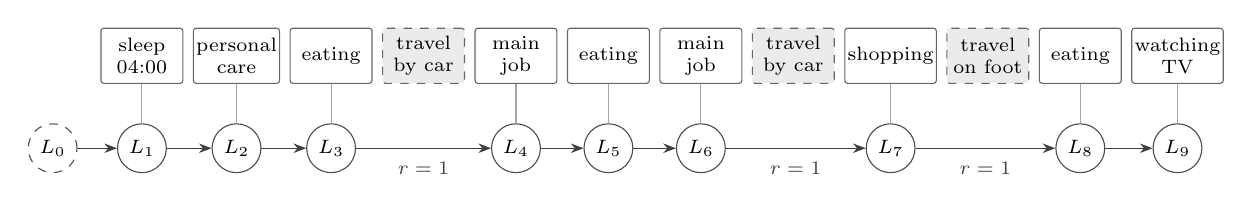
\begin{tikzpicture}[
      font=\scriptsize,
      act/.style={draw=black!60, rounded corners=1pt, minimum width=10.4mm, minimum height=7mm,
                  align=center, inner sep=1pt},
      trip/.style={act, dashed, fill=black!8},
      loc/.style={circle, draw=black!70, minimum size=6.2mm, inner sep=0pt},
      link/.style={-{Stealth[length=1.6mm]}, black!75},
      node distance=1.2mm]
    \node[act] (a1) {sleep\\04:00};
    \node[act, right=of a1] (a2) {personal\\care};
    \node[act, right=of a2] (a3) {eating};
    \node[trip, right=of a3] (t1) {travel\\by car};
    \node[act, right=of t1] (a4) {main\\job};
    \node[act, right=of a4] (a5) {eating};
    \node[act, right=of a5] (a6) {main\\job};
    \node[trip, right=of a6] (t2) {travel\\by car};
    \node[act, right=of t2] (a7) {shopping};
    \node[trip, right=of a7] (t3) {travel\\on foot};
    \node[act, right=of t3] (a8) {eating};
    \node[act, right=of a8] (a9) {watching\\TV};
    \foreach \i in {1,...,9} {
      \node[loc, below=5mm of a\i] (l\i) {$L_{\i}$};
      \draw[black!35] (a\i) -- (l\i);
    }
    \node[loc, dashed, left=5mm of l1] (l0) {$L_0$};
    \draw[link] (l0) -- (l1);
    \foreach \i/\j in {1/2, 2/3, 4/5, 5/6, 8/9} { \draw[link] (l\i) -- (l\j); }
    \foreach \i/\j in {3/4, 6/7, 7/8} { \draw[link] (l\i) -- node[below=0.5mm, font=\scriptsize] {$r = 1$} (l\j); }
  \end{tikzpicture}
  \caption{Imputation of the locations of an example diary. Activity episodes (boxes) are recorded, as is transport with its mode (shaded). The locations of the other episodes, $L_1$ to $L_9$, are drawn in temporal order, each from its distribution given the location drawn for the previous episode, the activity, the hour at which the episode starts, whether transport separates it from the previous episode ($r = 1$) and the respondent's age band. $L_0$ is the start state of the diary.}
  \label{fig:chain}
\end{figure}

Locations are drawn at random from the estimated distributions rather than set to their most probable class. For a single episode the most probable class maximises the expected accuracy, but it assigns the frequent locations to every episode for which they are the most likely and the rarer ones to none, which distorts the distribution of locations. Random draws reproduce that distribution in expectation. For Germany we draw 20 sets of locations from the main specification estimated on all 13 donors. Twenty are more than enough for the mean: among the combinations of the global analysis of Section~\ref{sec:uncertainty} that draw at random, a single set of draws accounts, including its interactions, for at most 0.3\% of the variance of any German daily total and for at most 0.7\% of that of the share at home in any ten-minute slot (1.4\% on weekdays), and the mean of 20 sets reduces the variance due to the draws twentyfold. Because the model is estimated only once, these are not proper multiple imputations in the sense of \textcite{rubinMultipleImputationNonresponse1987}: their spread reflects the randomness of the draws but not the uncertainty of the estimated probabilities or of their transfer to Germany. The leave-one-country-out errors measure the latter, and Section~\ref{sec:uncertainty} describes how they enter the uncertainty analysis.

The main specification combines three components: the unit to which a location is assigned, the variables on which the location probabilities are conditioned, and the rule that turns probabilities into locations. To see what each contributes, we compare it with variants that change one or more of them (Fig.~\ref{fig:components}). Two baselines place every episode outside transport at home or give it the most frequent location of its activity. Two slot-level variants draw a location independently for every ten-minute slot, given the activity and the slot ($t$ in place of $h$), with or without the age band. An episode-level variant draws one location per episode given the activity, the starting hour and the age band but not the previous location. The Markov variants omit the age band, use it as in \eqref{eq:markov}, or add the day type as a fifth level, and the modal version of the main specification assigns the most likely class at every step of the chain.

\begin{figure}[ht]
  \centering
  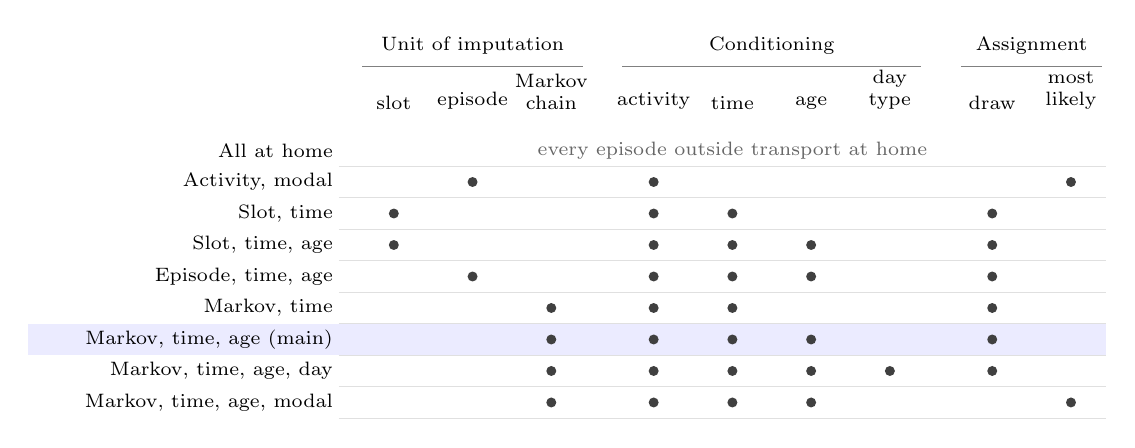
\begin{tikzpicture}[
      font=\scriptsize, x=1cm, y=1cm,
      dot/.style={circle, fill=black!75, inner sep=0pt, minimum size=3.6pt},
      head/.style={align=center, anchor=south}]
    % column positions: unit (slot, episode, chain), conditioning (activity, time, age, day type),
    % assignment (draw, most likely)
    \foreach \x/\lab in {0.6/slot, 1.6/episode, 2.6/{Markov\\chain}, 3.9/activity, 4.9/time,
                         5.9/age, 6.9/{day\\type}, 8.2/draw, 9.2/{most\\likely}} {
      \node[head] at (\x, 0.05) {\lab};
    }
    \foreach \x/\y/\lab in {0.6/2.6/{Unit of imputation}, 3.9/6.9/Conditioning, 8.2/9.2/Assignment} {
      \node[anchor=south] at ({(\x+\y)/2}, 0.75) {\lab};
      \draw[black!50] (\x-0.4, 0.72) -- (\y+0.4, 0.72);
    }
    \fill[blue!8] (-4.05, -2.95) rectangle (9.65, -2.55);
    \foreach \i/\lab in {1/{All at home}, 2/{Activity, modal}, 3/{Slot, time}, 4/{Slot, time, age},
                         5/{Episode, time, age}, 6/{Markov, time}, 7/{Markov, time, age (main)},
                         8/{Markov, time, age, day}, 9/{Markov, time, age, modal}} {
      \node[anchor=east] at (-0.05, -0.4*\i + 0.05) {\lab};
      \draw[black!12] (-0.1, -0.4*\i - 0.15) -- (9.65, -0.4*\i - 0.15);
    }
    \node[black!60] at (4.9, -0.35) {every episode outside transport at home};
    % rows: 2 activity modal, 3-4 slot, 5 episode, 6-9 Markov
    \foreach \i/\x in {2/1.6, 2/3.9, 2/9.2,
                       3/0.6, 3/3.9, 3/4.9, 3/8.2,
                       4/0.6, 4/3.9, 4/4.9, 4/5.9, 4/8.2,
                       5/1.6, 5/3.9, 5/4.9, 5/5.9, 5/8.2,
                       6/2.6, 6/3.9, 6/4.9, 6/8.2,
                       7/2.6, 7/3.9, 7/4.9, 7/5.9, 7/8.2,
                       8/2.6, 8/3.9, 8/4.9, 8/5.9, 8/6.9, 8/8.2,
                       9/2.6, 9/3.9, 9/4.9, 9/5.9, 9/9.2} {
      \node[dot] at (\x, -0.4*\i + 0.05) {};
    }
  \end{tikzpicture}
  \caption{Components of the main specification (shaded) and of the variants compared with it in Section~\ref{sec:res_variants}. Unit of imputation: a location is drawn for every ten-minute slot, for every activity episode independently, or for every episode in a Markov chain that also conditions on the previous location and on whether transport lies in between. Conditioning: the variables of the smoothing hierarchy, each entering as one level, in the order shown. Assignment: a random draw from the estimated distribution or the most likely class. All variants use $\alpha = 5$. Part A of the global sensitivity analysis (Section~\ref{sec:uncertainty}) crosses all units, the use or not of time, age and day type, both assignment rules and three values of $\alpha$, 144 combinations in all.}
  \label{fig:components}
\end{figure}

\subsection{Evaluation metrics}
\label{sec:metrics}

We evaluate each imputation with seven metrics, defined in Table~\ref{tab:metrics}. Energy demand models use time-use diaries both in aggregate and as sequences of occupancy \parencite{richardsonHighresolutionDomesticBuilding2008,widenCombinedMarkovchainBottomup2009,aertsMethodIdentificationModelling2014}, and the metrics cover both uses: the first three measure agreement slot by slot, the next three the distribution of locations over the day, and the last the number of location changes within diaries. Because two thirds or more of the slots are at home in every country, accuracy rewards imputations that favour the home, which Cohen's $\kappa$ corrects for. All metrics are computed for each held-out country over its slots with a recorded place and are summarised by their unweighted mean across countries. They come from one imputation per held-out country and variant. To show which places are recovered, Section~\ref{sec:res_places} also breaks agreement down by place, with the recall and precision of each place, the two components of macro-F1.

\begin{table}[ht]
  \centering
  \footnotesize
  \caption{Evaluation metrics, computed for each held-out country. Notation: $S$, the $N$ slots with a recorded place (transport excluded); $y_{dt}$ and $\hat y_{dt}$, the recorded and imputed class of slot $t$ of diary $d$; $n_{kl}$, the number of slots of $S$ recorded in class $k$ and imputed in class $l$, with row and column sums $n_{k\cdot}$ and $n_{\cdot l}$; $\mathcal{K}$, the places recorded in the country; $s_{tk}$ and $\hat s_{tk}$, the recorded and imputed share of respondents in class $k$ at slot $t = 1, \dots, 144$, weighted with WGHT1, with $h$ the home; $\pi_{uk}$ and $\hat\pi_{uk}$, their means over the six slots of hour $u$, for the places and transport; $c_d$ and $\hat c_d$, the number of pairs of consecutive slots of $S$ in diary $d$ with different classes, averaged over the $D$ diaries as $\bar c$ and $\bar{\hat c}$. The best value is 1 for the first three metrics and 0 for the others.}
  \label{tab:metrics}
  \begin{tabularx}{\textwidth}{@{}>{\raggedright\arraybackslash}p{2.9cm}>{\raggedright\arraybackslash}p{3.2cm}Lc@{}}
    \toprule
    Metric & What it measures & Definition & Weighted \\
    \midrule
    Accuracy & agreement slot by slot & $p_o = \frac{1}{N} \sum_{(d,t) \in S} \mathbf{1}[\hat y_{dt} = y_{dt}] = \frac{1}{N} \sum_k n_{kk}$ & no \\[3pt]
    Cohen's $\kappa$ \parencite{cohenCoefficientAgreementNominal1960} & agreement beyond chance & $\kappa = \dfrac{p_o - p_e}{1 - p_e}$, \quad $p_e = \dfrac{1}{N^2} \sum_k n_{k\cdot}\, n_{\cdot k}$ & no \\[6pt]
    Macro-F1 & agreement for every place, rare ones included & $\dfrac{1}{|\mathcal{K}|} \sum_{k \in \mathcal{K}} \dfrac{2 R_k P_k}{R_k + P_k}$, \quad recall $R_k = \dfrac{n_{kk}}{n_{k\cdot}}$, precision $P_k = \dfrac{n_{kk}}{n_{\cdot k}}$ ($P_k = 0$ if $n_{\cdot k} = 0$) & no \\
    \addlinespace
    Home share error (MAE, pp) & occupancy over the day & $\dfrac{100}{144} \sum_{t=1}^{144} \lvert \hat s_{th} - s_{th} \rvert$ & yes \\[6pt]
    Home share bias (pp) & systematic over- or understatement of occupancy & $\dfrac{100}{144} \sum_{t=1}^{144} (\hat s_{th} - s_{th})$ & yes \\[6pt]
    Hourly total variation distance (TVD) & distribution over all locations, as the share of respondents to be moved & $\dfrac{1}{24} \sum_{u=1}^{24} \dfrac{1}{2} \sum_k \lvert \hat\pi_{uk} - \pi_{uk} \rvert$ & yes \\
    \addlinespace
    Change error (\%) & number of location changes & $100 \left( \bar{\hat c} / \bar c - 1 \right)$, \quad $\bar c = \dfrac{1}{D} \sum_d c_d$ & no \\
    \bottomrule
  \end{tabularx}
\end{table}

The recall and precision of a place in one country rest on the respondents recorded at, or imputed to, that place, who can be few for rare places in small countries. Eurostat's guidelines for publishing results from the scientific use files bar results based on fewer than 20 respondents and require results based on 20 to 49 to be flagged \parencite{eurostatGuidelinesPublication2026}. We therefore report the recall and precision of individual countries only where at least 50 respondents stand behind them in every country, and otherwise only their means over countries.

\subsection{Uncertainty and sensitivity analysis}
\label{sec:uncertainty}

The German estimates are uncertain because locations are drawn at random, because the model rests on choices that could reasonably have been made otherwise, because the coding of the diaries can be read in more than one way, and because location patterns are transferred from the donor countries to Germany. We assess these sources together, in a global uncertainty and sensitivity analysis \parencite{saltelliGlobalSensitivityAnalysis2008b}. Varying one source at a time around a main specification explores a small part of the space of possible analyses and misses the interactions between them \parencite{saltelliHowAvoidPerfunctory2010}. We therefore varied the choices and assumptions at once, treating them as uncertain inputs in their own right, as in the modelling of the modelling process \parencite{lopianoUnpackingModelingProcess2024,saltelliMathematicalModelsState2025} and in multiverse analysis \parencite{steegenIncreasingTransparencyMultiverse2016}. Every factor takes a few discrete values, which we treated as equally plausible, so the full factorial design can be enumerated. Its functional analysis of variance gives exactly, rather than as Monte Carlo estimates, the first-order Sobol' index of each factor $X_i$, $S_i = V[E(Y \mid X_i)]/V(Y)$, the share of the variance of an output $Y$ that $X_i$ explains on its own, and its total index, $S_{Ti} = E[V(Y \mid X_{\sim i})]/V(Y)$, which adds the share due to its interactions with the other factors \parencite{sobolGlobalSensitivityIndices2001,hommaImportanceMeasuresGlobal1996}. One minus the sum of the first-order indices is the share of the variance due to interactions. The analysis has two parts (Fig.~\ref{fig:design}), which vary the same choices of method but differ in their outputs. In part A the outputs are the evaluation metrics of Section~\ref{sec:metrics}, which measure how well the imputation recovers locations that were recorded. In part B they are features of the imputed German diaries themselves: the hours per day at each location, the number of location changes per diary and the share of respondents at home in each slot.

The first part concerns the method (part A). Its factors are the unit of imputation (slot, episode, or episode in a Markov chain), the use or not of the time of day, the age band and the day type, the assignment rule (random draw or most likely class) and $\alpha$ (1, 5 or 20). Their 144 combinations include all variants of Fig.~\ref{fig:components} except the all-at-home baseline, which involves no choice that could be varied and serves only as the reference against which the metrics are read. Each combination is trained and validated as in Section~\ref{sec:design}: it is estimated on 12 donors and scored on the 13th, in turn for each of the 13 donors. The outputs are the seven metrics of Table~\ref{tab:metrics}, each averaged over the 13 validation countries. Besides the Sobol' indices of each metric, we compute the optimal-transport index of \textcite{borgonovoGlobalSensitivityAnalysis2025}, which measures how far fixing a factor moves the whole distribution of a metric rather than its mean or variance alone (Supporting Material~\ref{sec:appendix_indices}). No combination need be best on every metric, so we also identify the Pareto-optimal combinations, those that no other combination matches or beats on all seven, with the home share bias and the change error counted by their distance from zero.

The second part concerns the German estimates (part B). It crosses the same 144 combinations of method choices with three factors that arise only for Germany: an assumption about the coding of the diaries, the randomness of the draws and the transfer error. The coding assumption concerns code 13, which combines other places with locations the diarist did not specify. For activities that the donors carry out almost only at home, code 13 more likely means that the location was not specified. It is therefore either kept as recorded or treated as missing in the donor diaries for the 36 activities whose donor slots with a specified place (codes 1 to 7) are at home in at least 95\% of cases, with at least 1,000 such slots and with code 13 in at most 15\% of all their donor slots. Three further activities meet the first two conditions, but code 13 takes 41\% to 56\% of their donor slots, which points to other places rather than to unspecified ones. The randomness of the draws has ten levels, ten independent streams of random numbers, each used in every combination of the other factors. The most likely class involves no draw, so its ten levels give the same imputation. The transfer error has 13 levels, the errors (imputed minus recorded) made for each donor in part A under the same method choices, when it is imputed from the other 12. Subtracting one of them from the German estimate treats Germany as exchangeable with the donors and removes from each combination the systematic error it makes on them. These errors are taken with code 13 as recorded, since the held-out diaries cannot show which reading of the German coding is right.

The $144 \times 2 \times 10 = 2{,}880$ combinations of the first eight factors give one German imputation each, and with the 13 transfer errors 37,440 values of each output, each kept within its possible range. The share at home is analysed for all diaries and separately for weekdays and weekend days, with the donor errors taken from the same groups. We report the range spanned by the middle 90\% of these values as the uncertainty of the German estimates, together with the first-order and total indices, and locate within it the values of the combinations whose method choices are Pareto-optimal in part A.

\begin{figure}[ht]
  \centering
  \def\nohyphens{\hyphenpenalty=10000\relax}
  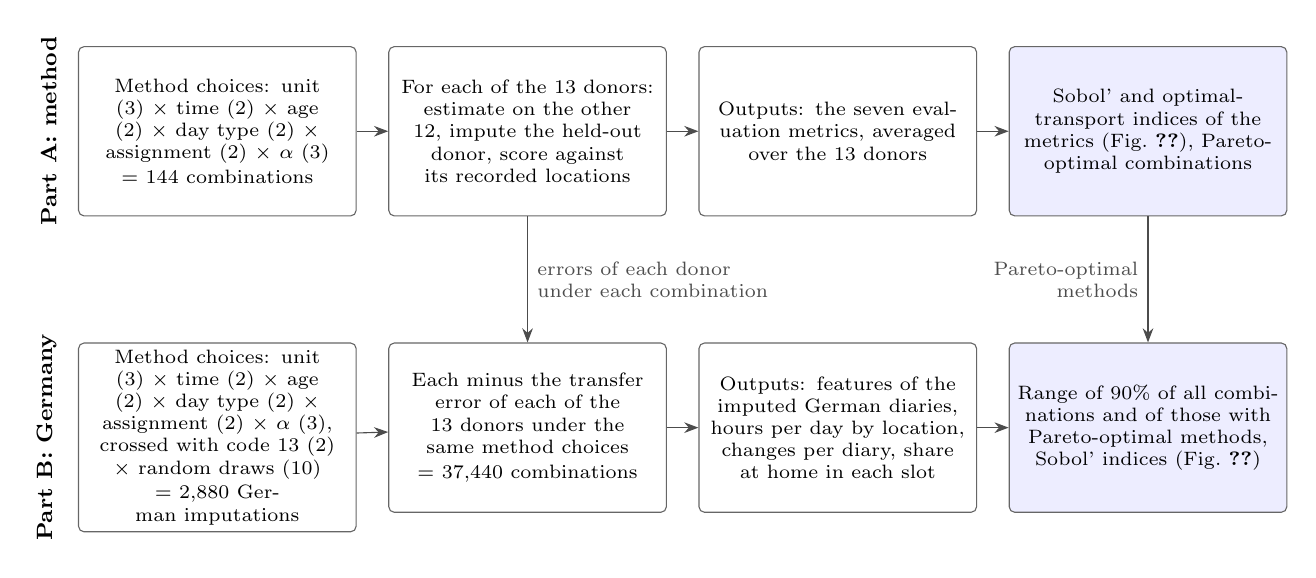
\begin{tikzpicture}[
      font=\scriptsize,
      box/.style={draw=black!60, rounded corners=2pt, align=center, text width=3.35cm, minimum height=2.15cm,
                  inner sep=2.5pt, execute at begin node=\nohyphens},
      res/.style={box, fill=blue!7},
      arr/.style={-{Stealth[length=1.8mm]}, black!70},
      part/.style={font=\footnotesize\bfseries, rotate=90, anchor=south}]
    \node[box] (a1) {Method choices: unit (3) $\times$ time (2) $\times$ age (2) $\times$ day type (2) $\times$ assignment (2) $\times$ $\alpha$ (3)\\[1pt] $=$ 144 combinations};
    \node[box, right=4mm of a1] (a2) {For each of the 13 donors: estimate on the other 12, impute the held-out donor, score against its recorded locations};
    \node[box, right=4mm of a2] (a3) {Outputs: the seven evaluation metrics, averaged over the 13 donors};
    \node[res, right=4mm of a3] (a4) {Sobol' and optimal-transport indices of the metrics (Fig.~\ref{fig:gsa_methods}), Pareto-optimal combinations};
    \node[box, below=16mm of a1] (b1) {Method choices: unit (3) $\times$ time (2) $\times$ age (2) $\times$ day type (2) $\times$ assignment (2) $\times$ $\alpha$ (3), crossed with code 13 (2) $\times$ random draws (10)\\[1pt] $=$ 2,880 German imputations};
    \node[box, below=16mm of a2] (b2) {Each minus the transfer error of each of the 13 donors under the same method choices\\[1pt] $=$ 37,440 combinations};
    \node[box, below=16mm of a3] (b3) {Outputs: features of the imputed German diaries, hours per day by location, changes per diary, share at home in each slot};
    \node[res, below=16mm of a4] (b4) {Range of 90\% of all combinations and of those with Pareto-optimal methods, Sobol' indices (Fig.~\ref{fig:gsa_germany})};
    \foreach \x/\y in {a1/a2, a2/a3, a3/a4, b1/b2, b2/b3, b3/b4} { \draw[arr] (\x) -- (\y); }
    \draw[arr] (a2) -- node[right, align=left, font=\scriptsize] {errors of each donor\\under each combination} (b2);
    \draw[arr] (a4) -- node[left, align=right, font=\scriptsize] {Pareto-optimal\\methods} (b4);
    \node[part] at ([xshift=-1.5mm]a1.west) {Part A: method};
    \node[part] at ([xshift=-1.5mm]b1.west) {Part B: Germany};
  \end{tikzpicture}
  \caption{Design of the global sensitivity analysis. Both parts vary the same 144 combinations of method choices. Part A estimates each combination on 12 donor countries and scores it on the 13th, for every donor, and its outputs are the evaluation metrics. Part B imputes Germany with each combination, under two readings of code 13 and with ten streams of random draws, and its outputs are features of the imputed diaries, from which the errors made for each donor in part A under the same method choices are subtracted (the 13 levels of the transfer error). The combinations that are Pareto-optimal in part A are then located in the distribution of the German estimates. Both designs are full factorials, so the Sobol' indices are computed exactly. Numbers in brackets are the levels of each factor.}
  \label{fig:design}
\end{figure}

\section{Results}
\label{sec:results}

\subsection{Activity, time and sequence}
\label{sec:res_variants}

Table~\ref{tab:variants} and Fig.~\ref{fig:variants} summarise the leave-one-country-out results for the 13 donor countries, each imputed from the other 12. Placing every episode outside transport at home is correct for 77.0\% of the scored slots on average, the level against which accuracy has to be read. The activity code carries most of the information: giving each episode the most frequent location of its activity raises accuracy to 0.902 and $\kappa$ to 0.731. Every variant that draws locations at random is less accurate than this modal rule, because a draw matches the recorded location less often than the most probable class does. The modal version of the main specification has the highest accuracy and $\kappa$ of all variants (0.908 and 0.750), and its accuracy exceeds that of the random draw by 0.026 to 0.042 in each of the 13 donor countries.

\begin{table}[ht]
  \centering
  \small
  \setlength{\tabcolsep}{4pt}
  \caption{Leave-one-country-out results by imputation variant, unweighted means over the 13 donor countries, each imputed from the other 12. The seven metrics of Table~\ref{tab:metrics}, computed over the slots with a recorded place, transport excluded. Home share error and bias: mean absolute and mean signed difference between the imputed and the recorded weighted share of respondents at home over the 144 ten-minute slots, in percentage points. Hourly TVD: total variation distance between the imputed and the recorded weighted distributions over locations, averaged over the 24 hours. Change error: relative difference between the imputed and the recorded mean number of location changes per diary (recorded: 3.48 on average). Time is the ten-minute slot in the slot-level variants and the hour in which the episode starts otherwise. All variants use $\alpha = 5$. In bold, the best value of each metric: the highest for the first three, the lowest for the home share error and the hourly TVD, and the closest to zero for the home share bias and the change error.}
  \label{tab:variants}
  % <<< generated: tab_variants >>>
\sisetup{detect-weight=true}
\begin{tabular}{l S[table-format=1.3] S[table-format=1.3] S[table-format=1.3] S[table-format=2.2] S[table-format=-1.2] S[table-format=1.3] S[table-format=-3.1]}
\toprule
Variant & {Accuracy} & {$\kappa$} & {Macro-F1} & {\makecell{Home share\\error (pp)}} & {\makecell{Home share\\bias (pp)}} & {\makecell{Hourly\\TVD}} & {\makecell{Change\\error (\%)}} \\
\midrule
\multicolumn{8}{l}{Baselines} \\
\quad All at home & 0.770 & 0.000 & 0.109 & 23.08 & 23.08 & 0.231 & -100.0 \\
\quad Activity, modal & 0.902 & 0.731 & 0.485 & 4.31 & 4.10 & 0.052 & 26.0 \\
\addlinespace
\multicolumn{8}{l}{Random draw} \\
\quad Slot, time & 0.852 & 0.614 & 0.451 & 2.72 & 1.13 & 0.035 & 521.5 \\
\quad Slot, time, age & 0.854 & 0.621 & 0.456 & 2.62 & \bfseries 0.91 & 0.034 & 510.7 \\
\quad Episode, time, age & 0.851 & 0.600 & 0.444 & 3.41 & 2.55 & 0.041 & 60.9 \\
\quad Markov, time & 0.872 & 0.666 & 0.487 & 2.64 & 1.48 & 0.034 & 9.4 \\
\quad Markov, time, age & 0.874 & 0.672 & 0.491 & 2.54 & 1.21 & 0.033 & 8.9 \\
\quad Markov, time, age, day & 0.874 & 0.673 & 0.493 & \bfseries 2.46 & 1.26 & \bfseries 0.032 & 8.8 \\
\addlinespace
\multicolumn{8}{l}{Modal assignment} \\
\quad Markov, time, age, modal & \bfseries 0.908 & \bfseries 0.750 & \bfseries 0.538 & 3.85 & 3.75 & 0.043 & \bfseries -3.5 \\
\bottomrule
\end{tabular}
% <<< end of tab_variants >>>
\end{table}

The modal versions buy this accuracy by distorting the distribution of locations. They assign the frequent locations to every episode for which these are the most likely and almost never assign the rare ones. The modal version of the main specification places 0.02\% of the scored slots at second homes or hotels, against 1.5\% in the recorded diaries, and it overstates the share of respondents at home at every time of day in 13 of the 16 held-out countries and in more than half of the slots in the other three (Fig.~\ref{fig:home_error} in the Supporting Material). Its home share error is 3.85 percentage points (pp) and its bias $+3.75$~pp, against 2.54~pp and $+1.21$~pp for the random draw. The activity-modal baseline errs in the same direction (error 4.31~pp, bias $+4.10$~pp).

\begin{figure}[ht]
  \centering
  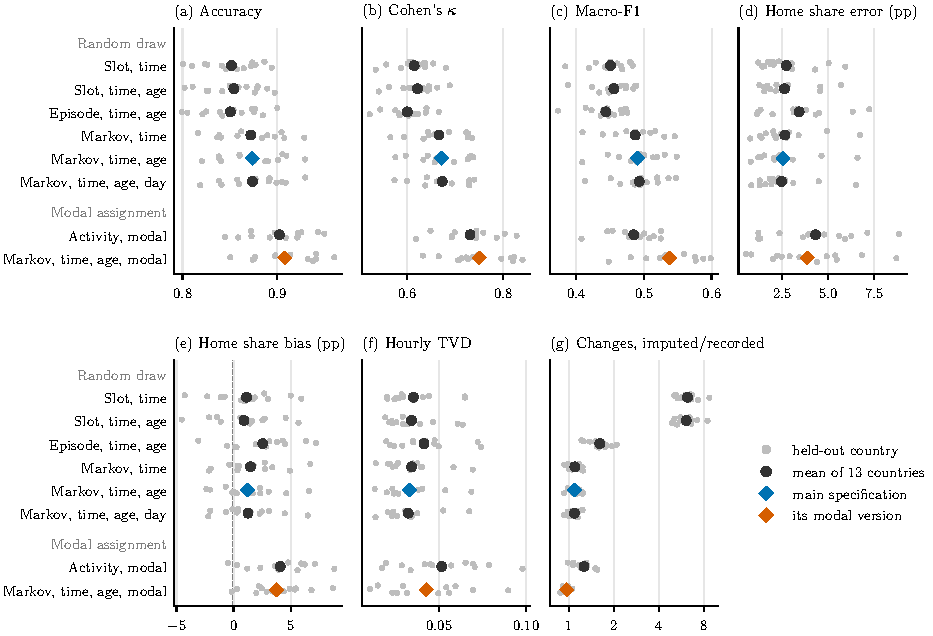
\includegraphics[width=\textwidth]{figures/fig_variants.pdf}
  \caption{Leave-one-country-out performance of the imputation variants for the 13 donor countries, each imputed from the other 12, on the seven evaluation metrics of Table~\ref{tab:metrics}. Grey dots are the held-out countries and larger markers their unweighted mean. In (g), the change error is shown as the mean number of location changes per diary, imputed divided by recorded, on a log scale (a ratio of 1.09 is a change error of $+9\%$), since random draws for every slot multiply the number of changes by five to nine. Dashed lines: no bias in (e), as many changes as recorded in (g). The all-at-home baseline is omitted (see Table~\ref{tab:variants}).}
  \label{fig:variants}
\end{figure}

How the draws are organised matters at least as much as what they condition on. Drawing a location independently for every ten-minute slot reproduces the share of respondents at home almost as well as the Markov chain (error 2.72~pp with time and 2.62~pp with time and age), since each slot is drawn from the distribution for its own activity and time. The imputed sequences, however, are unrealistic. The diaries change location 21 times a day on average, against 3.48 recorded changes, between five and nine times as often depending on the country. Such diaries cannot serve where the sequence matters, for instance to derive periods of occupancy or the number of journeys between places. Drawing one location per episode removes most of the spurious changes (5.48 per diary), but its accuracy (0.851) and home share error (3.41~pp) are worse than those of the slot-level draws. The Markov chain over episodes improves on both. With time and age it reaches an accuracy of 0.874 and a $\kappa$ of 0.672, higher than the slot-level draws in each of the 13 countries, and it produces 3.75 changes per diary, a change error of $+9\%$ on average, with country ratios between 0.93 and 1.23. Its home share error (2.54~pp) and hourly total variation distance (0.033) are close to those of the slot-level draws (2.62~pp and 0.034).

Once activity, time and sequence are known, the respondent's age and the day type add little. Adding the age band to the Markov chain changes accuracy by 0.002 and lowers the home share error from 2.64 to 2.54~pp, an improvement in 11 of the 13 countries. Adding the day type leaves accuracy unchanged and lowers the error slightly further, to 2.46~pp, in 8 of the 13 countries.

The global analysis of the method extends these comparisons to all 144 combinations of the components (Fig.~\ref{fig:gsa_methods}, Table~\ref{tab:gsa_methods}). The assignment rule accounts on its own for 92\% of the variance of accuracy, 64\% of that of the home share error and 56\% of that of the hourly total variation distance. The unit of imputation accounts for 42\% of the variance of the change error on its own and for 76\% including its interactions, nearly all of them with the assignment rule: drawing a location for every slot at random raises the number of changes by 518\% on average over the other components, while with the most likely class the change error lies between $-4\%$ (Markov chain) and $+32\%$ (slots). Together with their interaction, the unit and the assignment rule explain between 91\% (hourly total variation distance) and almost 100\% (change error) of the variance of each metric. The time of day accounts for at most 5.9\% of the variance of any metric, including its interactions, and the age band, the day type and $\alpha$ for at most 2.1\% each. Once the activity is known, the quality of the imputed diaries therefore depends on how locations are drawn rather than on which further variables condition them, whatever the choices of conditioning and smoothing. For every metric, the optimal-transport index ranks the assignment rule and the unit of imputation first, in the same order as the Sobol' indices, and it orders the other factors as the total index does for six of the seven metrics; for the home share bias, it swaps the age band and $\alpha$, whose total indices are 1.1\% and 1.2\%. Its value lies between half the first-order index and the total index, and near the total index where a factor acts mostly through its interactions, as the unit of imputation and the assignment rule do on the change error (73\% and 53\%, against first-order indices of 42\% and 24\% and total indices of 76\% and 58\%). No combination is best on all seven metrics. Nineteen of the 144 are Pareto-optimal, and all are Markov chains (Fig.~\ref{fig:pareto} in the Supporting Material): ten draw at random, and among them are the combinations with the smallest home share error, bias and hourly total variation distance, while nine assign the most likely class, and among them are those with the highest accuracy, $\kappa$ and macro-F1 and the change error closest to zero. The main specification is one of the ten.

\begin{figure}[ht]
  \centering
  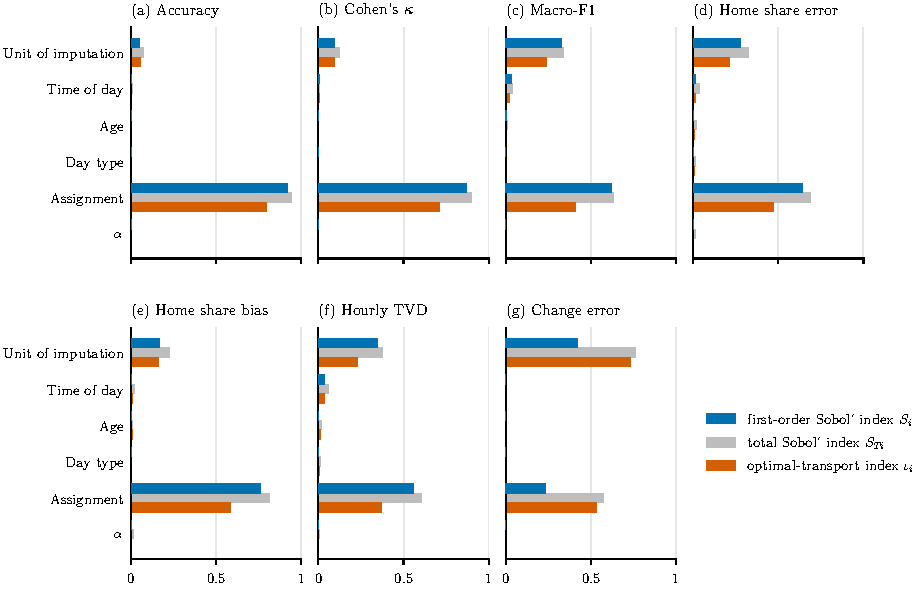
\includegraphics[width=\textwidth]{figures/fig_gsa_methods.pdf}
  \caption{Global sensitivity analysis of the method (part A): first-order and total Sobol' indices and optimal-transport index of each component over the 144 combinations of the unit of imputation (slot, episode, Markov chain), the use of time, age and day type, the assignment rule (random draw or most likely class) and $\alpha$ (1, 5, 20), for the seven evaluation metrics of Table~\ref{tab:metrics}, each averaged over the 13 donor countries (values in Table~\ref{tab:gsa_methods} of the Supporting Material).}
  \label{fig:gsa_methods}
\end{figure}

For Austria, France and Luxembourg, scored on the classes they record, the variants rank by accuracy essentially as for the donors: 0.882 for the main specification, against 0.868 for the slot-level draws with age and 0.916 for the modal version. The home share error is smaller in these countries for all random-draw variants (1.13 to 1.87~pp). The main specification reproduces the share at home slightly better than the slot-level draws (1.15 against 1.20~pp), and adding the age band lowers its error from 1.21 to 1.15~pp.

The errors differ between countries in a systematic way (Section~\ref{sec:res_countries} of the Supporting Material). Accuracy largely follows the time spent at home, from 0.820 in Finland to 0.929 in Romania. The imputation pulls each country toward the average of the donors, overstating the time at home where respondents spend less time there and understating it where they spend more. The largest errors arise for Finland and Norway, where much time is spent at second homes and at other people's homes, which the imputed diaries assign mostly to the main home.

\subsection{Recoverable and unrecoverable locations}
\label{sec:res_places}

Fig.~\ref{fig:places} breaks the results down by location. The main specification recovers the home, the workplace or school, and shops and services well, with mean recall of 0.94, 0.88 and 0.84 and precision of 0.93, 0.91 and 0.80. These locations are tied to particular activities, such as sleep and personal care, paid work and study, and shopping. Other people's homes, restaurants, cafes and pubs, and other or unspecified places are recovered less reliably (recall of 0.42, 0.27 and 0.60), because the activities carried out there, such as eating, socialising and leisure, also take place at home. Second homes and hotels are in practice not recovered (recall of 0.02 and 0.01). A day at a holiday home or a hotel may consist of the same activities as a day at home, and the diary rarely contains anything that indicates where the respondent slept. The random draw still reproduces the aggregate time at most locations (Fig.~\ref{fig:places}a): other people's homes account for 0.80 hours a day in both the recorded and the imputed diaries, restaurants, cafes and pubs for 0.23 and 0.21 hours, and shops and services for 0.30 and 0.32 hours. Second homes are reproduced worst (0.19 hours recorded, 0.10 hours imputed), and hotels are also underrepresented (0.10 against 0.08 hours). The use of second homes is concentrated in Estonia, Finland and Norway (0.41 to 0.69 hours a day), and the remaining donors cannot reproduce it when these countries are held out.

\begin{figure}[ht]
  \centering
  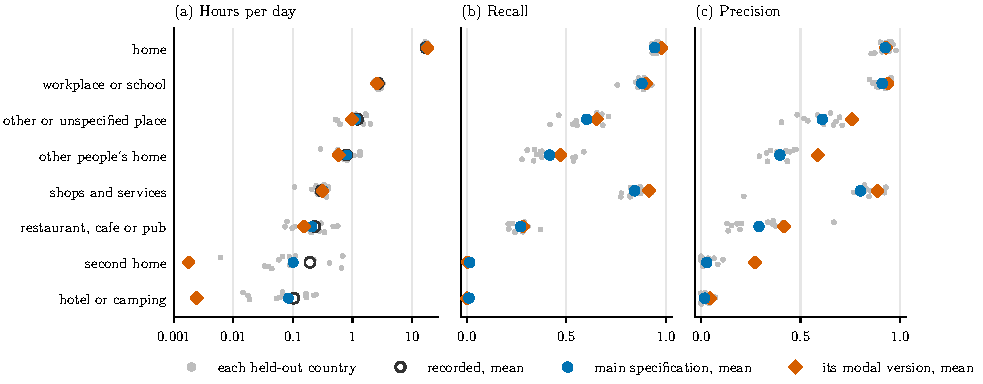
\includegraphics[width=\textwidth]{figures/fig_places.pdf}
  \caption{Leave-one-country-out results by location for the main specification and its modal version, 13 donor countries. (a) Weighted hours per day recorded and imputed at each location (log scale). (b) Recall, the share of the slots recorded at a location that are imputed there. (c) Precision, the share of the slots imputed at a location that were recorded there. Grey dots are the individual countries, with recorded hours in (a) and the main specification in (b) and (c), where they are shown only for locations at which at least 50 respondents stand behind the score in every country (Section~\ref{sec:metrics}).}
  \label{fig:places}
\end{figure}

\subsection{Imputed locations for Germany}
\label{sec:res_germany}

Estimated on all 13 donors and applied to the 27,143 German diaries, the main specification assigns on average 17.1 hours a day to the home, 2.5 hours to the workplace or school, 1.6 hours to other or unspecified places, 0.7 hours to other people's homes, 0.4 hours to shops and services and 0.3 hours to restaurants, cafes and pubs, with about 0.1 hours each at second homes and at hotels (Table~\ref{tab:germany}). The German diaries record a further 1.2 hours of transport. The imputed time at home falls in the middle of the range recorded in the other countries, from 15.4 hours in Norway to 19.0 hours in Romania, close to the 17.1 hours recorded in France, and the imputed share at home lies within the range of the recorded shares at every time of day (Fig.~\ref{fig:germany_home}a). The imputed diaries change location 4.2 times a day on average (unweighted, as for the held-out countries), within the range recorded in the other countries (2.2 to 4.4), and more often on weekdays (4.5) than at weekends (3.6).

\begin{table}[ht]
  \centering
  \small
  \setlength{\tabcolsep}{4pt}
  \caption{Imputed hours per day by location in the German diaries (2012/13), mean of 20 imputations with the main specification estimated on all 13 donors, weighted with WGHT1. Transport is recorded in the diaries, all other rows are imputed. Range: 5th to 95th percentile over the 37,440 combinations of method choices, coding assumption, random draws and transfer errors of the global sensitivity analysis (all), and over those whose method choices are Pareto-optimal in part A (Pareto; Section~\ref{sec:res_uncertainty}).}
  \label{tab:germany}
  % <<< generated: tab_germany >>>
\begin{tabular}{l S[table-format=2.2] c c S[table-format=2.2] S[table-format=2.2] S[table-format=2.2] S[table-format=2.2] S[table-format=2.2]}
\toprule
 & \multicolumn{3}{c}{All respondents} & \multicolumn{2}{c}{Day type} & \multicolumn{3}{c}{Age (years)} \\
\cmidrule(lr){2-4} \cmidrule(lr){5-6} \cmidrule(lr){7-9}
Location & {Imputed} & {\makecell{Range,\\all}} & {\makecell{Range,\\Pareto}} & {Weekdays} & {Weekend} & {10--17} & {18--64} & {65+} \\
\midrule
Home & 17.07 & 15.65--17.77 & 15.70--17.78 & 16.36 & 18.56 & 16.18 & 16.31 & 19.73 \\
Second home & 0.11 & 0.01--0.69 & 0.01--0.70 & 0.10 & 0.13 & 0.12 & 0.11 & 0.12 \\
Other people's home & 0.71 & 0.44--1.20 & 0.46--1.17 & 0.62 & 0.89 & 1.02 & 0.70 & 0.62 \\
Hotel or camping & 0.10 & 0.01--0.24 & 0.02--0.25 & 0.09 & 0.11 & 0.11 & 0.10 & 0.06 \\
Workplace or school & 2.54 & 2.39--2.89 & 2.46--3.07 & 3.47 & 0.54 & 3.07 & 3.24 & 0.16 \\
Shops and services & 0.44 & 0.13--0.47 & 0.13--0.48 & 0.46 & 0.39 & 0.21 & 0.44 & 0.51 \\
Restaurant, cafe or pub & 0.28 & 0.13--0.61 & 0.16--0.52 & 0.23 & 0.39 & 0.20 & 0.31 & 0.22 \\
Other or unspecified place & 1.56 & 1.19--2.18 & 1.16--2.04 & 1.40 & 1.91 & 1.84 & 1.49 & 1.67 \\
Transport & 1.21 & recorded & recorded & 1.27 & 1.08 & 1.25 & 1.30 & 0.90 \\
\midrule
Diaries & {27{,}143} &  &  & {17{,}469} & {9{,}674} & {4{,}714} & {18{,}723} & {3{,}706} \\
\bottomrule
\end{tabular}
% <<< end of tab_germany >>>
\end{table}

\begin{figure}[ht]
  \centering
  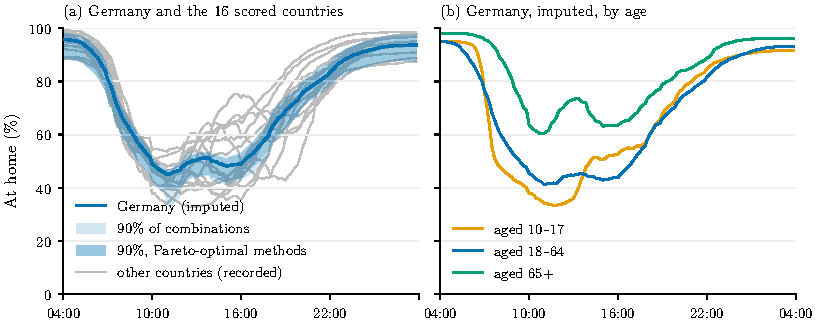
\includegraphics[width=\textwidth]{figures/fig_germany_home.pdf}
  \caption{(a) Share of German respondents at home by time of day, imputed with the main specification (blue), and recorded share at home in the 16 countries with location data (grey). The shaded ranges contain 90\% of the 37,440 combinations of the global sensitivity analysis in each slot (light) and 90\% of those whose method choices are Pareto-optimal in part A (dark; Section~\ref{sec:res_uncertainty}). (b) Imputed share at home by age group.}
  \label{fig:germany_home}
\end{figure}

The imputed profiles follow the timing of activities in the German diaries (Fig.~\ref{fig:germany_tempogram}). On weekdays the share at home falls to 36\% at 11:00, when 40\% of respondents are at a workplace or school. On weekend days it reaches its minimum of 55\% at 16:00, when 19.5\% of respondents are at other or unspecified places, 10.2\% are in transport and 6.4\% are at other people's homes. Respondents aged 65 and over spend 19.7 hours a day at home, against 16.2 and 16.3 hours in the two younger groups, and those aged 10 to 17 spend the most time at other people's homes (1.0 hours a day).

\begin{figure}[ht]
  \centering
  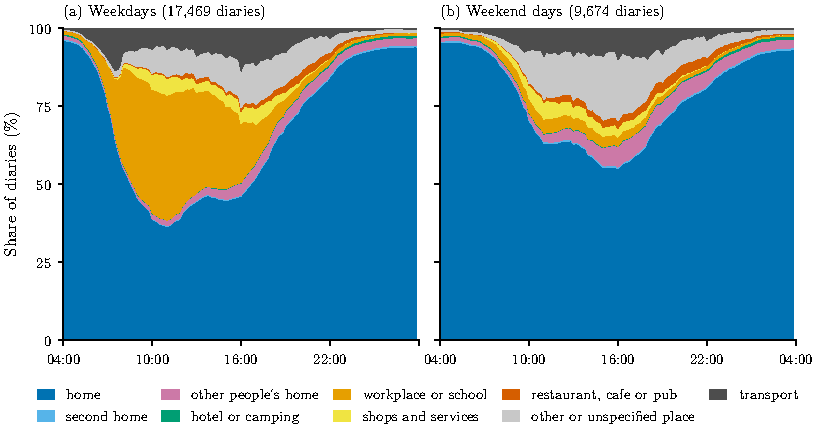
\includegraphics[width=\textwidth]{figures/fig_germany_tempogram.pdf}
  \caption{Location of the German respondents by time of day on (a) weekdays and (b) weekend days, mean of 20 imputations with the main specification, weighted with WGHT1. Transport is recorded in the diaries, all other locations are imputed.}
  \label{fig:germany_tempogram}
\end{figure}

\subsection{Uncertainty and sensitivity of the German estimates}
\label{sec:res_uncertainty}

Over the 37,440 combinations of the global analysis, the German time at home lies between 15.7 and 17.8 hours a day (5th to 95th percentile), the time at the workplace or school between 2.4 and 2.9 hours and the time at other or unspecified places between 1.2 and 2.2 hours (Table~\ref{tab:germany}). The number of location changes per diary lies between 3.4 and 5.5. The combinations are centred below the main specification for the time at home (median 16.7 hours, against 17.1), because the imputation overstated it in most donors (Table~\ref{tab:countries} in the Supporting Material), and close to it for the number of changes (median 4.2). The transfer error accounts for 92\% of the variance of the time at home on its own and 96\% including its interactions, and for between 74\% and 99.8\% of that of the other daily totals on its own (Fig.~\ref{fig:gsa_germany}, Table~\ref{tab:gsa_germany}). The six method choices of part A together account for 2.7\% of the variance of the time at home, 3.4\% of that of the time at the workplace or school, 16\% of that of the time at other or unspecified places and 28\% of that of the number of changes, and for 7\%, 19\%, 23\% and 63\% including their interactions with the other factors, mostly with the transfer error. Assigning the most likely class to slots or to independent episodes places more time at other or unspecified places than the other combinations of unit and assignment rule (medians of 1.75 and 1.81 hours, against 1.48 to 1.53).

For the number of location changes, the method choices matter as much as the transfer error. The unit of imputation accounts for 19.2\% of its variance on its own and 53.6\% including its interactions, the transfer error for 32.5\% and 54.8\%. The two interact because the donor errors are large for slot-level draws, which impute between 15.8 and 19.2 changes per diary more than recorded, and differ more between donors than those of the Markov chain. Corrected by them, the German estimates lie between 3.0 and 6.7 changes per diary with slot-level draws (5th to 95th percentile) and between 3.4 and 4.4 with the Markov chain and random draws.

The random draws account for at most 0.2\% of the variance of any German daily total and for at most 0.4\% of that of the share at home in any slot (0.6\% on weekdays), including their interactions, and for about twice as much among the combinations that draw at random. This is why the spread across repeated imputations says so little about the uncertainty (Section~\ref{sec:discussion}). Treating code 13 as missing for home activities moves on average 0.1 hours a day from other or unspecified places to the home, 0.2 hours with the main specification, and accounts for 2.6\% of the variance of the time at other or unspecified places and 4.4\% of that of the number of changes on its own, and for 4.5\% and 16.8\% including its interactions. The time of day, the age band, the day type and $\alpha$ each account for less than 1\% of the variance of every daily total and of the number of changes on their own, and for at most 4.3\% including their interactions.

By time of day, the range of the share at home is narrowest at 10:00 (7.6~pp) and widest at 11:20 (13.3~pp; Fig.~\ref{fig:germany_home}a), where imputations of slots or independent episodes, mostly with the most likely class and corrected by the errors made for Norway and Finland, give the lowest values. The transfer error accounts for at least 66\% of the variance of the share at home in every slot on its own and for at least 84\% including its interactions (57\% and 81\% on weekdays; Fig.~\ref{fig:gsa_home}). Its share is lowest at 14:30, where the unit of imputation accounts for 10\% of the variance on its own and 24\% including its interactions. Interactions account for up to 23\% of the variance in a slot (29\% on weekdays).

\begin{figure}[ht]
  \centering
  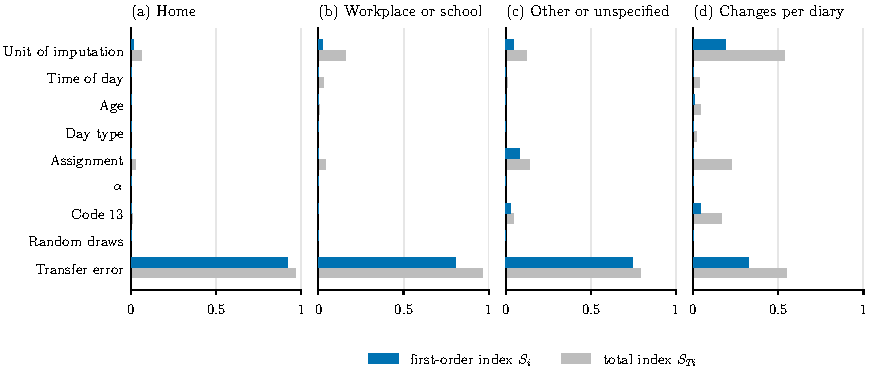
\includegraphics[width=\textwidth]{figures/fig_gsa_germany.pdf}
  \caption{Global sensitivity analysis of the German estimates (part B): first-order and total Sobol' indices over the 37,440 combinations of the method choices of part A (unit of imputation, use of time, age and day type, assignment rule, $\alpha$), the treatment of code 13 for home activities, ten streams of random draws and the transfer error of each of the 13 donors under the same method choices. Hours per day (a) at home, (b) at the workplace or school and (c) at other or unspecified places, and (d) number of location changes per diary (all daily totals in Table~\ref{tab:gsa_germany} of the Supporting Material).}
  \label{fig:gsa_germany}
\end{figure}

The 19 combinations of method choices that are Pareto-optimal in part A, crossed with the coding assumption, the draws and the transfer errors, give 4,940 combinations. Over these, the time at home lies between 15.7 and 17.8 hours, almost the same range as over all combinations, with a median of 17.0 hours, and the other daily totals vary over ranges of similar width, slightly higher for the workplace or school (2.5 to 3.1 hours; Table~\ref{tab:germany}). The number of changes lies between 3.5 and 4.3, a narrower range between the 9th and the 59th percentile of all combinations, as none of the 19 imputes slots or independent episodes. Within these combinations, the transfer error accounts for 96\% of the variance of the time at home and 87\% of that of the number of changes on its own, and the method choices for 0.7\% and 3.3\%. The main specification alone gives between 15.7 and 17.8 hours at home and between 3.5 and 4.4 changes per diary over its 260 combinations of coding assumption, draws and transfer errors. For the share at home, the range over the Pareto-optimal combinations is 9.1~pp wide on average over the day, against 10.0~pp over all combinations, and at most 10.9~pp, at 18:40 (Fig.~\ref{fig:germany_home}a). As the Pareto-optimal combinations are selected on the same 13 donors whose errors make up the transfer error, the narrower ranges they give, for the number of changes and on average for the share at home, are conditional on that selection and may understate the uncertainty for a country outside the donor pool.

The 1.6 hours at other or unspecified places in the main specification inherit the mixed content of code 13, which combines other specified places with locations the diarists did not specify, so part of this time stands for unspecified locations rather than for other places. The time at second homes and hotels follows the donor pattern whatever the German diaries contain, so German use of holiday homes or hotels above the donor average would be counted as time at home, as it was for Finland and Norway.

\section{Discussion}
\label{sec:discussion}

Most of what a time-use diary reveals about where people are lies in what they are doing. Assigning each episode the most frequent location of its activity recovers 90\% of the recorded slots in the 13 donor countries, against 77\% when everyone is placed at home. Time of day, the previous location and the trips between episodes add the structure that the activity alone misses, such as eating at home in the morning and evening but elsewhere at midday, or returning home after the last trip of the day. Once these are known, age and the day of the week add little. In-sample evaluations, in which the location probabilities are estimated from the same diaries that are then imputed, would suggest otherwise, because splitting a cell can only raise the expected agreement of random draws within it, the sum of the squared location probabilities. Holding out whole countries removes this advantage and shows which conditioning variables carry information that transfers.

Once the activity and the time of day are known, the way locations are drawn matters more than what else they are conditioned on. Assigning the most likely location maximises the share of correctly imputed slots, but it erases rare locations and inflates the time at home, by about 0.9 hours a day on average across the donors. Applications that use imputed diaries in aggregate, such as occupancy profiles for energy demand models, need the distribution of locations to be right, and random draws from the estimated distributions provide it. Drawing each ten-minute slot independently gets the aggregate shares about right but produces some 21 location changes per diary instead of 3.5, so the imputed diaries consist of implausibly short stays. Occupancy models derive the length and timing of absences from such sequences \parencite{richardsonHighresolutionDomesticBuilding2008,widenCombinedMarkovchainBottomup2009,aertsMethodIdentificationModelling2014,kleinebrahmUsingNeuralNetworks2021}, and slot-by-slot imputation distorts exactly these quantities. Treating activity episodes as the unit of imputation and linking them in a Markov chain keeps the number of changes within 9\% of the recorded one on average and raises accuracy as well. Supervised machine learning has been used to infer whether respondents are at home when diaries do not report it \parencite{araoInferringHomeOutofhome2025}. Any such classifier faces the same choice: predicting the most likely location for each unit inherits the distortions of modal assignment, while sampling slot by slot inherits those of independent draws. In the global analysis of the method, which crosses the unit of imputation and the assignment rule with all combinations of conditioning variables and smoothing, the assignment rule and the unit of imputation together account for between 91\% and almost 100\% of the variance of each evaluation metric, and the age band, the day type and $\alpha$ for at most 2.1\% each. Every combination that no other matches or beats on all seven metrics is a Markov chain over episodes, and the choice among them is one between random draws, which keep the distribution of locations, and the most likely class, which maximises agreement slot by slot.

The imputation rests on the assumption that, given the activity sequence, the time of day and age, German respondents are at the same locations as respondents in the donor countries. This assumption cannot be tested on the German data, but the held-out countries show how it fails elsewhere. The errors are systematic. The imputation pulls each country toward the average of its donors, overstating the time at home where respondents spend less time there and understating it where they spend more. The largest errors arise for Finland and Norway, where much time is spent at second homes and at other people's homes. A day at a summer cottage may consist of the same activities as a day at home, and the diary rarely contains anything that tells the two apart. Germany's recorded activities place its imputed time at home in the middle of the range of the donors, but whether its use of holiday homes, hotels or other people's homes also matches the donor average cannot be checked on the diaries of 2012/13, a point we return to below.

Differences in coding between surveys also limit what can be imputed. Code 13 of the scientific use files combines other specified places with locations the diarist did not specify, so the imputed time at other or unspecified places mixes the two. Treating code 13 as missing for home activities shifts time from this class to the home, 0.2 hours a day with the main specification, and in the global analysis it accounts for 4.5\% of the variance of the German time at other or unspecified places including its interactions, against at most 0.4\% for each of $\alpha$, the age band and the day type, and for 11\% over the combinations with Pareto-optimal methods. Three countries record only some of the places. Most donors also record a mode of transport for some activities other than trips, which the German diaries almost never do, and we have counted every slot with a recorded mode as transport, in the donor diaries as well, so that reading on a train is time in transport, as the trip itself is. If some German respondents recorded such time under the other activity without a mode, the imputation places it at home or elsewhere. The time concerned is small: the donors record on average about 0.1 hours a day of other activities with a recorded mode of transport, and the United Kingdom, which records the most, about 0.4 hours. Location codes that keep unspecified locations apart from other places, and a location for every slot, would make future rounds of HETUS more useful for energy research and easier to complete where locations are missing.

Multiple imputation treats the spread across imputations as the uncertainty of the imputed values \parencite{rubinMultipleImputationNonresponse1987,vanbuurenFlexibleImputationMissing2012}. For locations transferred between countries, this spread captures little of the actual error. When we imputed each held-out country 20 times with the main specification, plain 95\% predictive intervals from the spread across imputations, $\bar{x} \pm t_{0.975,19}\, s \sqrt{1 + 1/20}$ with $\bar{x}$ and $s$ the mean and standard deviation across imputations, contained the recorded share at home in only 14\% of the slots. Twenty imputations are enough to show this. They estimate the spread across imputations to within about 16\%, the relative standard error of a standard deviation estimated from 20 draws, $1/\sqrt{2 \cdot 19}$, whereas the intervals would have to be more than ten times wider to contain 95\% of the recorded values. Proper multiple imputation would also draw the model parameters, but the dominant error lies in the transfer between countries, which parameter draws from the pooled donors do not represent. The global analysis therefore treats the transfer error as a factor of its own, next to the randomness of the draws, the modelling choices and the coding assumption, and apportions the variance of the German estimates among all of them. The transfer error accounts for 92\% of the variance of the time at home on its own and 74\% to over 99\% of that of the other daily totals, the random draws for at most 0.2\% of that of any of them, and the choices, the assumption and the interactions for the rest, so the uncertainty of the time spent at each place lies mainly in the transfer. Varying one choice at a time around the main specification would show the effect of each choice but not this balance, nor the interactions, which matter here. Interactions account for 42\% of the variance of the German number of location changes and for up to 23\% of that of the share at home in a slot (29\% on weekdays). The unit of imputation, which accounts for 19\% of the variance of the number of changes on its own, accounts for 54\% including its interactions, 19 points of which involve the transfer error: how far the donors' errors spread depends on the unit, and for slot-level draws they spread most. Where statistical matching bounds the uncertainty left by the conditional independence assumption \parencite{contiUncertaintyAnalysisStatistical2012}, the errors of the held-out donors give it an empirical distribution, at the price of assuming that Germany's transfer error resembles one of those of the 13 donors. With 13 donors, its range is itself estimated with some error.

For models that derive building occupancy and energy demand from time-use diaries \parencite{torritiReviewTimeUse2014,lopianoEnergyDemandIts2022}, the imputed German diaries provide daily rhythms and sequences of locations consistent with those recorded elsewhere in Europe. On weekdays the share at home falls to 36\% in the late morning, when 40\% of respondents are at a workplace or school, and rises again as paid work and study end. In 90\% of the combinations of the global analysis with Pareto-optimal methods the weekday share at home at 11:00 lies between 31\% and 38\%, and in 90\% of all combinations between 24\% and 37\%, the lowest values coming from imputations of slots or independent episodes, mostly with the most likely class, corrected by the errors made for Norway and Finland. Ranges of this size should be carried into occupancy-based estimates of residential and non-residential demand, for instance by running a demand model on the imputed diaries and reporting its results together with the range implied by the transfer errors. Modal assignment, which might seem the natural choice for a single best guess, overstates home occupancy and should be avoided. Time at second homes and hotels, and the corresponding absences from the main home, is not recovered and needs other sources where it matters, such as in holiday periods or in regions with many second homes.

The evaluation rests on the 16 countries with location data, and Germany may differ from all of them in ways that matter for location. A direct test requires German diaries with recorded locations. The 2012/13 diary asked for the mode of transport but not for the place of activities. Its successor, the German time use survey of 2022 in the 2020 round of HETUS, records the place of every activity in the categories of the HETUS 2018 guidelines, with unspecified places kept apart from other places. Eurostat's tables for this survey give 17.2 hours a day at home and 2.2 hours at the workplace or school for respondents aged 10 and over \parencite{eurostatTimeSpentMain2026}, against 17.1 and 2.5 hours imputed here for 2012/13. The 2022 values for the home, other people's homes, second homes, shops and restaurants fall within the ranges of the global analysis (Table~\ref{tab:germany}), while the time at the workplace or school falls below its range, which may reflect the spread of working from home after 2020. The 0.3 hours a day at second homes in 2022, against 0.1 hours imputed, also hint at more use of holiday homes in Germany than in the average donor country. With a decade, a pandemic and a new diary between the two surveys, these comparisons do not test the imputation. The national scientific use file of the 2022 survey \parencite{fdzZeitverwendungserhebung2022} allows such a test: removing its places, imputing them from the HETUS donors as for 2012/13 and comparing the result with the recorded places would measure the transfer error for German respondents directly, once the activity codes of 2022 are mapped onto the 2008 activity list. The harmonised microdata of the 2020 round of HETUS, which include the German survey of 2022, are not expected from Eurostat before 2027 \parencite{eurostatHETUSMicrodata2026}. With them, the test could be repeated within one round, with donors and target coded alike.

The model uses the activity sequence, time and age but not household composition, employment status or region, which may shape where people spend their time. The leave-one-country-out results suggest that such variables would add little once activity and sequence are known, as age and day type do, but they could matter for subgroups. Second homes and hotels would require a diary-level state, such as a day spent away from the main home, that the German file does not record. Finally, the global analysis varies one feature of the coding, the meaning of code 13. The treatment of modes of transport is fixed by the rule that every slot with a recorded mode is transport, and surveys also differ in how they code trips and secondary activities, which the evaluation takes as given.

Future work can build on the uncertainty estimates as much as on the imputed diaries. Extending the global analysis through an energy demand model, with the transfer error and the modelling choices of the demand model as further factors, would show how much each matters for estimates of peak load and demand flexibility, and the same leave-one-country-out design can assess the imputation of other variables that some HETUS countries do not collect.

\section{Conclusion}
\label{sec:conclusion}

Germany's contribution to the 2010 round of the Harmonised European Time Use Surveys lacks the locations of activities, which energy demand models need to place people at home, at work or elsewhere. We imputed these locations from the 13 countries that record all of them, with a Markov chain over activity episodes that conditions on the activity, the time of day, the previous location, intervening trips and age. We judged the result by imputing each donor from the other 12, and three countries that record only some places from all 13, and we apportioned the variance of the results among the randomness of the draws, the main modelling choices, a coding assumption and the error of transferring locations between countries in a global sensitivity analysis. The study has four take-home messages.

First, missing locations can be imputed from other countries' diaries with good aggregate accuracy, provided that the imputation respects the structure of the diary. Assigning one location to each activity episode and drawing the episodes in order keeps the number of location changes within 9\% of the recorded one on average, where drawing every ten-minute slot independently overstates it sixfold. Drawing from the estimated distributions keeps the time at home close to the recorded value and preserves part of the time at rare places, where assigning the most likely location overstates the time at home and erases the rare places.

Second, given the activity and the time of day, how locations are assigned matters more than which further variables condition them. Across the combinations of the global analysis, age, day type and the strength of smoothing each explain at most 2.1\% of the variance of any evaluation metric, while the assignment rule and the unit of imputation together explain 93\% of that of the home share error and almost all of that of the error in the number of location changes. No combination is best on every metric, and those that no other matches or beats on all of them are Markov chains over episodes, with random draws or the most likely class.

Third, for a country imputed from others, the uncertainty of the time spent at each place lies in the transfer between countries rather than in the randomness of the draws or in the modelling choices. Plain intervals from repeated imputations contain the recorded share at home in only 14\% of the slots of the held-out countries, and the transfer error accounts for 92\% of the variance of the German time at home on its own and 96\% including its interactions. The modelling choices matter for the number of location changes, and restricting them to the Pareto-optimal ones narrows its range from 3.4--5.5 to 3.5--4.3 changes per diary. Users of imputed diaries should carry the transfer uncertainty into their models rather than the spread of repeated imputations.

Fourth, some locations cannot be recovered from activities at all. Time at second homes and at hotels is imputed as time at home or elsewhere, and code 13 of the scientific use files mixes other places with unspecified ones.

For Germany, the imputed diaries place respondents at home for 17.1 hours a day, with 90\% of the combinations of the global analysis between 15.7 and 17.8 hours, at a workplace or school for 2.5 hours and at other or unspecified places for 1.6 hours, with daily rhythms that follow the recorded activities. A decade later, the German survey of 2022, which records locations, gives 17.2 hours at home. The imputed diaries can serve energy demand and occupancy models, provided that the transfer uncertainty is carried along with them.

\section*{Data and code availability}

This paper is based on data from Eurostat, Harmonised European Time Use Surveys, 2010 round. The responsibility for all conclusions drawn from the data lies entirely with the author. The scientific use files are available from Eurostat to recognised research entities for approved research projects and cannot be redistributed. The imputed German diaries are derived from these files and fall under the same conditions, but researchers with access to the files can recreate them with the code and the random seeds recorded with it. The code, the settings of the runs reported here, the aggregate results behind all tables and figures, and the script that produces the figures and tables from these results are available
at \url{https://github.com/Confareneoclassico/tus-location-imputation}.
In line with Eurostat's guidelines for publishing results from the scientific use files \parencite{eurostatGuidelinesPublication2026}, no statistic reported here or in the repository rests on fewer than 50 respondents.

\clearpage
\newpage

\printbibliography

% ===========================================================================
% Supporting Material
% ===========================================================================
\clearpage
\setcounter{section}{0}
\renewcommand{\thesection}{S\arabic{section}}
\renewcommand{\theHsection}{S\arabic{section}}
\setcounter{table}{0}
\renewcommand{\thetable}{S\arabic{table}}
\renewcommand{\theHtable}{S\arabic{table}}
\setcounter{figure}{0}
\renewcommand{\thefigure}{S\arabic{figure}}
\renewcommand{\theHfigure}{S\arabic{figure}}

\begin{center}
{\Large\bfseries Supporting Material}\\[4pt]
Imputation of missing locations in time-use surveys
\end{center}

\section{Transfer between countries}
\label{sec:res_countries}

Table~\ref{tab:countries} reports the main specification for each held-out country. Accuracy ranges from 0.820 in Finland to 0.929 in Romania and largely follows the time spent at home: across the 13 donors, its correlation with the accuracy of the all-at-home baseline is 0.89. Chance-corrected agreement depends less on the home share (correlation 0.62) and ranges among the donors from 0.575 in Finland to 0.738 in Romania.

\begin{table}[ht]
  \centering
  \footnotesize
  \setlength{\tabcolsep}{3.5pt}
  \caption{Leave-one-country-out results for the main specification (Markov, time, age) by held-out country. The 13 donor countries are imputed from the other 12, and Austria, France and Luxembourg from all 13 donors and scored on the classes they record, so that their macro-F1 is not comparable with that of the donors. The seven metrics of Table~\ref{tab:metrics}, with the accuracy of the all-at-home baseline for reference. Home share bias: mean over the 144 slots of the imputed minus the recorded weighted share at home. Change error: relative difference between the imputed and the recorded mean number of location changes per diary.}
  \label{tab:countries}
  % <<< generated: tab_countries >>>
\begin{tabular}{l r S[table-format=1.3] S[table-format=1.3] S[table-format=1.3] S[table-format=1.3] S[table-format=1.2] S[table-format=-1.2] S[table-format=1.3] S[table-format=-2.1]}
\toprule
Country & {Diaries} & {\makecell{All at home\\accuracy}} & {Accuracy} & {$\kappa$} & {Macro-F1} & {\makecell{Home share\\error (pp)}} & {\makecell{Home share\\bias (pp)}} & {\makecell{Hourly\\TVD}} & {\makecell{Change\\error (\%)}} \\
\midrule
\multicolumn{10}{l}{Full place coding (donors)} \\
\quad BE & 11{,}118 & 0.771 & 0.860 & 0.643 & 0.489 & 0.79 & 0.01 & 0.013 & 16.7 \\
\quad EE & 9{,}946 & 0.765 & 0.875 & 0.669 & 0.489 & 3.07 & 3.07 & 0.035 & 4.8 \\
\quad EL & 14{,}274 & 0.806 & 0.910 & 0.733 & 0.548 & 1.51 & 0.14 & 0.027 & -1.0 \\
\quad ES & 19{,}295 & 0.732 & 0.860 & 0.671 & 0.494 & 2.61 & 2.32 & 0.033 & -7.2 \\
\quad FI & 7{,}453 & 0.714 & 0.820 & 0.575 & 0.481 & 6.58 & 6.58 & 0.069 & 6.1 \\
\quad HU & 8{,}391 & 0.812 & 0.887 & 0.657 & 0.447 & 2.38 & -0.13 & 0.038 & 23.1 \\
\quad IT & 38{,}234 & 0.761 & 0.890 & 0.726 & 0.531 & 1.20 & 0.27 & 0.020 & 0.5 \\
\quad NL & 14{,}035 & 0.725 & 0.838 & 0.634 & 0.409 & 2.06 & 1.67 & 0.041 & 6.1 \\
\quad NO & 7{,}882 & 0.680 & 0.838 & 0.661 & 0.494 & 4.63 & 4.63 & 0.054 & 16.8 \\
\quad PL & 76{,}657 & 0.802 & 0.905 & 0.731 & 0.520 & 1.34 & -0.70 & 0.023 & -2.1 \\
\quad RO & 56{,}514 & 0.862 & 0.929 & 0.738 & 0.501 & 2.38 & -2.38 & 0.025 & 15.2 \\
\quad RS & 6{,}835 & 0.824 & 0.901 & 0.698 & 0.513 & 2.07 & -2.07 & 0.024 & 13.1 \\
\quad UK & 16{,}078 & 0.755 & 0.841 & 0.596 & 0.463 & 2.34 & 2.34 & 0.032 & 23.5 \\
\addlinespace
\multicolumn{10}{l}{Partial place coding (scored only)} \\
\quad AT & 8{,}234 & 0.734 & 0.898 & 0.740 & 0.870 & 1.07 & -0.18 & 0.011 & -0.8 \\
\quad FR & 27{,}699 & 0.775 & 0.851 & 0.605 & 0.479 & 1.19 & 0.61 & 0.018 & 13.2 \\
\quad LU & 4{,}162 & 0.747 & 0.896 & 0.753 & 0.663 & 1.20 & -0.33 & 0.020 & 7.2 \\
\bottomrule
\end{tabular}
% <<< end of tab_countries >>>
\end{table}

The share of respondents at home is reproduced to within 2~pp on average over the day in Belgium, Greece, Italy and Poland, and in the three partially coded countries. Most of the larger errors are systematic offsets that persist through the day (Fig.~\ref{fig:home_error}), and on average over the countries 95\% of the slots lie within $\pm 6.6$~pp of the recorded share. In Finland and Norway the imputation places too many respondents at home throughout the day and night, by 6.6 and 4.6~pp on average. Both countries record more time than any other donor at second homes (0.66 and 0.69 hours a day, against 0.11 hours on average in the other 11 donors) and at other people's homes (1.34 and 1.33 hours, against 0.70 hours), and 13\% and 11\% of their diaries start away from home, against between 1\% and 8\% in the other countries. The imputed diaries assign most of this time to the main home. Smaller positive biases appear in Estonia, the United Kingdom, Spain and the Netherlands (1.7 to 3.1~pp), and negative ones in Romania and Serbia ($-2.4$ and $-2.1$~pp), where respondents spend more time at home than in any other country. Across the 13 donors the bias falls as the time recorded at home rises (correlation $-0.89$), so the imputed home shares are pulled toward the average of the donor pool. In daily totals, the imputation overstates the time at home by 0.29 hours on average, with errors from $-0.57$ hours in Romania to $+1.58$ hours in Finland. Hungary is the exception: the imputation places too many respondents at home from about 06:40 to 16:10 and too few from then through the night, so a home share error of 2.38~pp comes with a bias close to zero. The change error lies between $-7\%$ in Spain and $+23\%$ in Hungary and the United Kingdom.

\begin{figure}[ht]
  \centering
  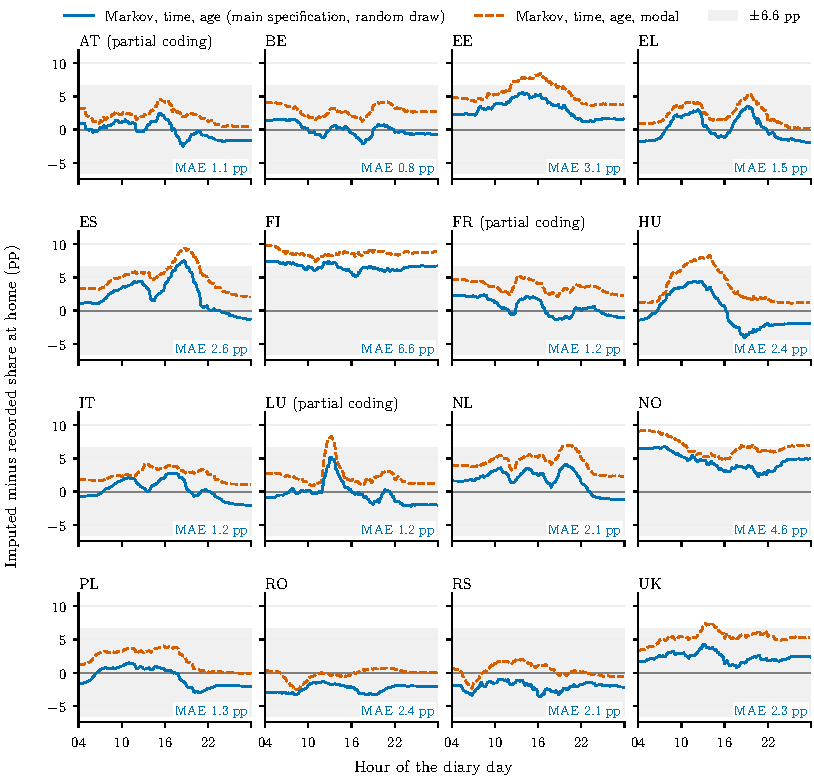
\includegraphics[width=\textwidth]{figures/fig_home_error.pdf}
  \caption{Imputed minus recorded weighted share of respondents at home by time of day for each held-out country, for the main specification (solid) and its modal version (dashed). The 13 donor countries are imputed from the other 12, and Austria, France and Luxembourg from all 13 donors. MAE: mean absolute error of the main specification over the 144 slots. Grey band: $\pm 6.6$~pp, within which 95\% of the slots of the held-out countries fall on average for the mean of 20 imputations per country (the curves show a single imputation).}
  \label{fig:home_error}
\end{figure}

\section{Sensitivity indices and Pareto-optimal combinations}
\label{sec:appendix_indices}

Table~\ref{tab:gsa_methods} gives the first-order and total Sobol' indices and the optimal-transport indices of the evaluation metrics of part A, and Table~\ref{tab:gsa_germany} the Sobol' indices of the German daily totals and number of changes of part B of the global sensitivity analysis (Section~\ref{sec:uncertainty} of the main text). Fig.~\ref{fig:gsa_methods} shows the indices of part A for all seven metrics, and Fig.~\ref{fig:gsa_germany} those of four of the German outputs. Fig.~\ref{fig:gsa_home} shows the first-order indices of the share of German respondents at home by time of day.

The optimal-transport index of \textcite{borgonovoGlobalSensitivityAnalysis2025} of factor $X_i$ for a metric $Y$ is
\begin{equation*}
\iota_i = \frac{E\left[W_2^2\left(P_Y, P_{Y \mid X_i}\right)\right]}{2 V(Y)},
\end{equation*}
where $W_2$ is the 2-Wasserstein distance between the distribution of $Y$ over all 144 combinations and its distribution over the combinations that share a level of $X_i$, and the expectation runs over the levels of $X_i$. The index is 0 when fixing $X_i$ leaves the distribution of $Y$ unchanged and 1 when $X_i$ determines $Y$. On the real line, the optimal transport between two distributions pairs their values in increasing order, so $W_2^2$ is the integral over $(0, 1)$ of the squared difference between their quantile functions. As every factor is discrete and the design is enumerated, the distances are exact: for a factor with $L$ levels, $W_2^2$ is the mean squared difference between the sorted values of the 144 combinations and the sorted values of the $144/L$ combinations of a level, each counted $L$ times.

The squared distance $W_2^2$ is the sum of the squared distance between the means and the squared distance between the centred distributions, so the index splits into half the first-order Sobol' index $S_i$, due to the shift of the mean, and a part due to changes in the spread and shape of the distribution. Since the factors are independent, pairing each combination with the one that differs from it only in the level of $X_i$ is a transport plan between the two distributions, whose mean squared distance, averaged over the levels, is $2 S_{Ti} V(Y)$. Hence $S_i/2 \le \iota_i \le S_{Ti}$. A factor that acts through its interactions changes the spread of a metric as well as its mean, which raises its index above half its first-order index, towards its total index.

We do not compute a joint index of the seven metrics, although \textcite{borgonovoGlobalSensitivityAnalysis2025} define the index for vector outputs as well. The metrics measure different things on different scales, so a joint index needs a common scale, which they do not have, and its value depends on the one chosen. For the assignment rule it lies between 57\% and 68\%, and for the unit of imputation between 27\% and 31\%, depending on whether the metrics are standardised, ranked or divided by their range, on whether $\kappa$ and macro-F1, whose correlations with accuracy over the 144 combinations are 0.99 and 0.90, are included, and on whether the change error enters in percent or as the logarithm of the ratio of imputed to recorded changes. Under each of these choices it ranks the assignment rule first, the unit of imputation second, then the time of day and the age band, with the day type and $\alpha$ below 1\%. The trade-offs between the metrics, which a joint index would add to the indices of the single metrics, are shown without a common scale by the Pareto-optimal combinations (Fig.~\ref{fig:pareto}).

\begin{table}[ht]
  \centering
  \footnotesize
  \setlength{\tabcolsep}{2.5pt}
  \caption{Global sensitivity analysis of the method (part A): (a) first-order ($S_i$) and (b) total ($S_{Ti}$) Sobol' indices and (c) optimal-transport indices ($\iota_i$) over the 144 combinations of the unit of imputation (slot, episode, Markov chain), the use of time, age and day type, the assignment rule (random draw or most likely class) and $\alpha$ (1, 5, 20), for each evaluation metric averaged over the 13 donor countries, in percent (of the variance of the metric for the Sobol' indices). Interactions: 100 minus the sum of the first-order indices.}
  \label{tab:gsa_methods}
  % <<< generated: tab_gsa_methods >>>
\begin{tabular}{l S[table-format=3.1] S[table-format=3.1] S[table-format=3.1] S[table-format=3.1] S[table-format=3.1] S[table-format=3.1] S[table-format=3.1]}
\toprule
Output & {Unit} & {Time} & {Age} & {Day type} & {Assignment} & {$\alpha$} & {\makecell{Inter-\\actions}} \\
\midrule
\multicolumn{8}{l}{(a) First-order indices $S_i$} \\
\quad Accuracy & 5.2 & 0.3 & 0.1 & 0.0 & 92.1 & 0.0 & 2.3 \\
\quad $\kappa$ & 9.3 & 0.4 & 0.1 & 0.0 & 86.8 & 0.0 & 3.4 \\
\quad Macro-F1 & 32.9 & 3.2 & 0.3 & 0.0 & 62.3 & 0.0 & 1.4 \\
\quad Home share error & 27.8 & 1.5 & 0.1 & 0.0 & 64.3 & 0.2 & 6.1 \\
\quad Home share bias & 16.8 & 0.0 & 0.1 & 0.1 & 75.8 & 0.3 & 6.9 \\
\quad Hourly TVD & 34.5 & 3.9 & 0.2 & 0.0 & 55.8 & 0.1 & 5.5 \\
\quad Change error & 42.3 & 0.0 & 0.0 & 0.0 & 23.6 & 0.0 & 34.1 \\
\addlinespace
\multicolumn{8}{l}{(b) Total indices $S_{Ti}$} \\
\quad Accuracy & 7.2 & 0.8 & 0.1 & 0.0 & 94.1 & 0.2 &  \\
\quad $\kappa$ & 12.3 & 0.8 & 0.2 & 0.1 & 90.0 & 0.1 &  \\
\quad Macro-F1 & 33.7 & 4.1 & 1.0 & 0.1 & 63.2 & 0.0 &  \\
\quad Home share error & 32.3 & 3.5 & 2.1 & 1.2 & 68.9 & 1.2 &  \\
\quad Home share bias & 22.8 & 1.8 & 1.1 & 0.5 & 81.5 & 1.2 &  \\
\quad Hourly TVD & 37.9 & 5.9 & 1.8 & 1.3 & 60.3 & 0.8 &  \\
\quad Change error & 76.4 & 0.0 & 0.0 & 0.0 & 57.7 & 0.0 &  \\
\addlinespace
\multicolumn{8}{l}{(c) Optimal-transport indices $\iota_i$} \\
\quad Accuracy & 5.4 & 0.6 & 0.1 & 0.0 & 79.6 & 0.1 &  \\
\quad $\kappa$ & 9.6 & 0.6 & 0.2 & 0.0 & 71.0 & 0.1 &  \\
\quad Macro-F1 & 24.2 & 2.4 & 0.4 & 0.1 & 40.9 & 0.0 &  \\
\quad Home share error & 21.1 & 1.6 & 0.9 & 0.6 & 46.9 & 0.2 &  \\
\quad Home share bias & 16.0 & 0.6 & 0.6 & 0.2 & 58.5 & 0.5 &  \\
\quad Hourly TVD & 23.2 & 3.5 & 1.1 & 0.7 & 37.3 & 0.2 &  \\
\quad Change error & 73.5 & 0.0 & 0.0 & 0.0 & 53.2 & 0.0 &  \\
\bottomrule
\end{tabular}
% <<< end of tab_gsa_methods >>>
\end{table}

\begin{table}[ht]
  \centering
  \footnotesize
  \setlength{\tabcolsep}{2.5pt}
  \caption{Global sensitivity analysis of the German estimates (part B): (a) first-order ($S_i$) and (b) total ($S_{Ti}$) Sobol' indices over the 37,440 combinations of the method choices of part A, the treatment of code 13 for home activities (as recorded or missing), ten streams of random draws and the transfer error of each of the 13 donors under the same method choices, in percent of the variance of the hours per day at each location and of the number of location changes per diary. Interactions: 100 minus the sum of the first-order indices.}
  \label{tab:gsa_germany}
  % <<< generated: tab_gsa_germany >>>
\begin{tabular}{l S[table-format=3.1] S[table-format=3.1] S[table-format=3.1] S[table-format=3.1] S[table-format=3.1] S[table-format=3.1] S[table-format=3.1] S[table-format=3.1] S[table-format=3.1] S[table-format=3.1]}
\toprule
Output & {Unit} & {Time} & {Age} & {\makecell{Day\\type}} & {\makecell{Assign-\\ment}} & {$\alpha$} & {\makecell{Code\\13}} & {\makecell{Random\\draws}} & {\makecell{Transfer\\error}} & {\makecell{Inter-\\actions}} \\
\midrule
\multicolumn{11}{l}{(a) First-order indices $S_i$} \\
\quad Home & 1.5 & 0.0 & 0.0 & 0.0 & 0.2 & 0.0 & 0.5 & 0.0 & 92.1 & 5.6 \\
\quad Second home & 0.0 & 0.0 & 0.0 & 0.0 & 0.0 & 0.0 & 0.0 & 0.0 & 99.8 & 0.2 \\
\quad Workplace or school & 2.3 & 0.0 & 0.1 & 0.0 & 0.1 & 0.0 & 0.0 & 0.0 & 80.7 & 16.8 \\
\quad Other people's home & 2.2 & 0.0 & 0.0 & 0.1 & 0.3 & 0.0 & 0.0 & 0.0 & 92.1 & 5.3 \\
\quad Restaurant, cafe or pub & 0.4 & 0.0 & 0.0 & 0.0 & 5.0 & 0.0 & 0.0 & 0.0 & 88.4 & 6.1 \\
\quad Shops and services & 0.2 & 0.0 & 0.0 & 0.0 & 0.0 & 0.0 & 0.0 & 0.0 & 99.0 & 0.8 \\
\quad Hotel or camping & 0.3 & 0.0 & 0.0 & 0.0 & 0.4 & 0.0 & 0.0 & 0.0 & 97.8 & 1.4 \\
\quad Other or unspecified place & 4.3 & 0.1 & 0.0 & 0.0 & 8.0 & 0.0 & 2.6 & 0.0 & 74.5 & 10.4 \\
\quad Changes per diary & 19.2 & 0.5 & 0.8 & 0.1 & 0.2 & 0.0 & 4.4 & 0.0 & 32.5 & 42.3 \\
\addlinespace
\multicolumn{11}{l}{(b) Total indices $S_{Ti}$} \\
\quad Home & 6.0 & 0.4 & 0.3 & 0.2 & 2.5 & 0.0 & 0.8 & 0.0 & 96.5 &  \\
\quad Second home & 0.1 & 0.0 & 0.0 & 0.0 & 0.1 & 0.0 & 0.0 & 0.0 & 99.9 &  \\
\quad Workplace or school & 16.0 & 3.2 & 0.6 & 0.3 & 4.0 & 0.1 & 0.0 & 0.1 & 96.5 &  \\
\quad Other people's home & 5.7 & 0.8 & 1.1 & 0.9 & 2.7 & 0.1 & 0.0 & 0.1 & 96.3 &  \\
\quad Restaurant, cafe or pub & 4.0 & 2.5 & 0.8 & 0.4 & 7.6 & 0.1 & 0.0 & 0.0 & 92.7 &  \\
\quad Shops and services & 0.5 & 0.1 & 0.0 & 0.0 & 0.7 & 0.0 & 0.0 & 0.0 & 99.6 &  \\
\quad Hotel or camping & 1.3 & 0.4 & 0.2 & 0.1 & 1.3 & 0.2 & 0.1 & 0.2 & 98.6 &  \\
\quad Other or unspecified place & 12.3 & 0.9 & 0.4 & 0.2 & 14.2 & 0.1 & 4.5 & 0.0 & 79.3 &  \\
\quad Changes per diary & 53.6 & 3.7 & 4.3 & 2.2 & 22.7 & 0.1 & 16.8 & 0.0 & 54.8 &  \\
\bottomrule
\end{tabular}
% <<< end of tab_gsa_germany >>>
\end{table}

\begin{figure}[ht]
  \centering
  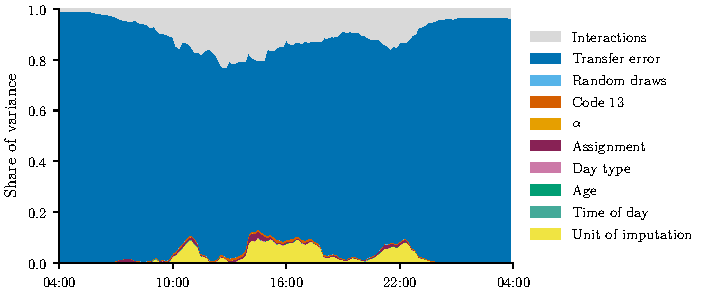
\includegraphics[width=0.75\textwidth]{figures/fig_gsa_home.pdf}
  \caption{Global sensitivity analysis of the German estimates (part B): share of the variance of the weighted share of German respondents at home in each ten-minute slot, all days, due to each factor alone (first-order Sobol' indices) and to interactions (1 minus their sum), over the 37,440 combinations.}
  \label{fig:gsa_home}
\end{figure}

\begin{figure}[ht]
  \centering
  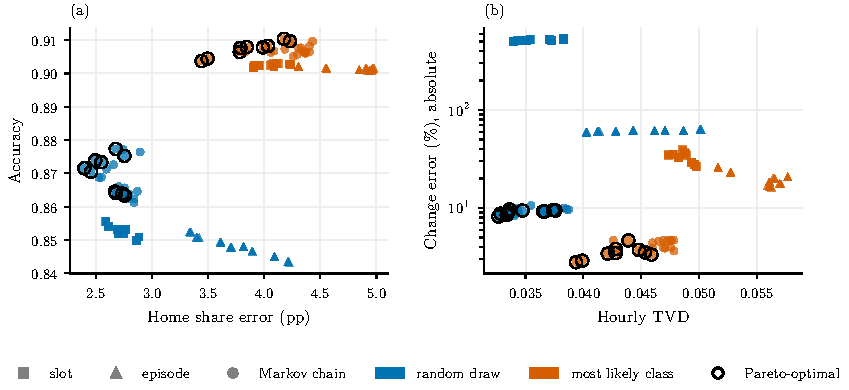
\includegraphics[width=\textwidth]{figures/fig_pareto.pdf}
  \caption{The 144 combinations of method choices of part A, by (a) home share error and accuracy and (b) hourly total variation distance and absolute change error (log scale), each averaged over the 13 donor countries. Colour: assignment rule. Marker: unit of imputation. Outlined: Pareto-optimal over all seven metrics.}
  \label{fig:pareto}
\end{figure}

\end{document}
